% Options for packages loaded elsewhere
\PassOptionsToPackage{unicode}{hyperref}
\PassOptionsToPackage{hyphens}{url}
\PassOptionsToPackage{dvipsnames,svgnames,x11names}{xcolor}
%
\documentclass[
]{article}

\usepackage{amsmath,amssymb}
\usepackage{lmodern}
\usepackage{iftex}
\ifPDFTeX
  \usepackage[T1]{fontenc}
  \usepackage[utf8]{inputenc}
  \usepackage{textcomp} % provide euro and other symbols
\else % if luatex or xetex
  \usepackage{unicode-math}
  \defaultfontfeatures{Scale=MatchLowercase}
  \defaultfontfeatures[\rmfamily]{Ligatures=TeX,Scale=1}
  \setmainfont[]{Latin Modern Roman}
  \setmathfont[]{Latin Modern Math}
\fi
% Use upquote if available, for straight quotes in verbatim environments
\IfFileExists{upquote.sty}{\usepackage{upquote}}{}
\IfFileExists{microtype.sty}{% use microtype if available
  \usepackage[]{microtype}
  \UseMicrotypeSet[protrusion]{basicmath} % disable protrusion for tt fonts
}{}
\makeatletter
\@ifundefined{KOMAClassName}{% if non-KOMA class
  \IfFileExists{parskip.sty}{%
    \usepackage{parskip}
  }{% else
    \setlength{\parindent}{0pt}
    \setlength{\parskip}{6pt plus 2pt minus 1pt}}
}{% if KOMA class
  \KOMAoptions{parskip=half}}
\makeatother
\usepackage{xcolor}
\setlength{\emergencystretch}{3em} % prevent overfull lines
\setcounter{secnumdepth}{5}
% Make \paragraph and \subparagraph free-standing
\ifx\paragraph\undefined\else
  \let\oldparagraph\paragraph
  \renewcommand{\paragraph}[1]{\oldparagraph{#1}\mbox{}}
\fi
\ifx\subparagraph\undefined\else
  \let\oldsubparagraph\subparagraph
  \renewcommand{\subparagraph}[1]{\oldsubparagraph{#1}\mbox{}}
\fi


\providecommand{\tightlist}{%
  \setlength{\itemsep}{0pt}\setlength{\parskip}{0pt}}\usepackage{longtable,booktabs,array}
\usepackage{calc} % for calculating minipage widths
% Correct order of tables after \paragraph or \subparagraph
\usepackage{etoolbox}
\makeatletter
\patchcmd\longtable{\par}{\if@noskipsec\mbox{}\fi\par}{}{}
\makeatother
% Allow footnotes in longtable head/foot
\IfFileExists{footnotehyper.sty}{\usepackage{footnotehyper}}{\usepackage{footnote}}
\makesavenoteenv{longtable}
\usepackage{graphicx}
\makeatletter
\def\maxwidth{\ifdim\Gin@nat@width>\linewidth\linewidth\else\Gin@nat@width\fi}
\def\maxheight{\ifdim\Gin@nat@height>\textheight\textheight\else\Gin@nat@height\fi}
\makeatother
% Scale images if necessary, so that they will not overflow the page
% margins by default, and it is still possible to overwrite the defaults
% using explicit options in \includegraphics[width, height, ...]{}
\setkeys{Gin}{width=\maxwidth,height=\maxheight,keepaspectratio}
% Set default figure placement to htbp
\makeatletter
\def\fps@figure{htbp}
\makeatother
\newlength{\cslhangindent}
\setlength{\cslhangindent}{1.5em}
\newlength{\csllabelwidth}
\setlength{\csllabelwidth}{3em}
\newlength{\cslentryspacingunit} % times entry-spacing
\setlength{\cslentryspacingunit}{\parskip}
\newenvironment{CSLReferences}[2] % #1 hanging-ident, #2 entry spacing
 {% don't indent paragraphs
  \setlength{\parindent}{0pt}
  % turn on hanging indent if param 1 is 1
  \ifodd #1
  \let\oldpar\par
  \def\par{\hangindent=\cslhangindent\oldpar}
  \fi
  % set entry spacing
  \setlength{\parskip}{#2\cslentryspacingunit}
 }%
 {}
\usepackage{calc}
\newcommand{\CSLBlock}[1]{#1\hfill\break}
\newcommand{\CSLLeftMargin}[1]{\parbox[t]{\csllabelwidth}{#1}}
\newcommand{\CSLRightInline}[1]{\parbox[t]{\linewidth - \csllabelwidth}{#1}\break}
\newcommand{\CSLIndent}[1]{\hspace{\cslhangindent}#1}

\usepackage{arxiv}
\usepackage{orcidlink}
\usepackage{amsmath}
\usepackage[T1]{fontenc}
\makeatletter
\makeatother
\makeatletter
\makeatother
\makeatletter
\@ifpackageloaded{caption}{}{\usepackage{caption}}
\AtBeginDocument{%
\ifdefined\contentsname
  \renewcommand*\contentsname{Table of contents}
\else
  \newcommand\contentsname{Table of contents}
\fi
\ifdefined\listfigurename
  \renewcommand*\listfigurename{List of Figures}
\else
  \newcommand\listfigurename{List of Figures}
\fi
\ifdefined\listtablename
  \renewcommand*\listtablename{List of Tables}
\else
  \newcommand\listtablename{List of Tables}
\fi
\ifdefined\figurename
  \renewcommand*\figurename{Figure}
\else
  \newcommand\figurename{Figure}
\fi
\ifdefined\tablename
  \renewcommand*\tablename{Table}
\else
  \newcommand\tablename{Table}
\fi
}
\@ifpackageloaded{float}{}{\usepackage{float}}
\floatstyle{ruled}
\@ifundefined{c@chapter}{\newfloat{codelisting}{h}{lop}}{\newfloat{codelisting}{h}{lop}[chapter]}
\floatname{codelisting}{Listing}
\newcommand*\listoflistings{\listof{codelisting}{List of Listings}}
\makeatother
\makeatletter
\@ifpackageloaded{caption}{}{\usepackage{caption}}
\@ifpackageloaded{subcaption}{}{\usepackage{subcaption}}
\makeatother
\makeatletter
\@ifpackageloaded{tcolorbox}{}{\usepackage[many]{tcolorbox}}
\makeatother
\makeatletter
\@ifundefined{shadecolor}{\definecolor{shadecolor}{rgb}{.97, .97, .97}}
\makeatother
\makeatletter
\makeatother
\ifLuaTeX
  \usepackage{selnolig}  % disable illegal ligatures
\fi
\IfFileExists{bookmark.sty}{\usepackage{bookmark}}{\usepackage{hyperref}}
\IfFileExists{xurl.sty}{\usepackage{xurl}}{} % add URL line breaks if available
\urlstyle{same} % disable monospaced font for URLs
\hypersetup{
  pdftitle={Assessing the validity of a calcifying oral biofilm model as a suitable proxy for dental calculus},
  pdfauthor={Bjørn Peare Bartholdy; Irina M. Velsko; Shira Gur-Arieh; Zandra Fagernäs; Amanda G. Henry},
  colorlinks=true,
  linkcolor={blue},
  filecolor={Maroon},
  citecolor={Blue},
  urlcolor={Blue},
  pdfcreator={LaTeX via pandoc}}

\newcommand{\runninghead}{A Preprint }
\renewcommand{\runninghead}{Validity of a calcifying oral biofilm
model }
\title{Assessing the validity of a calcifying oral biofilm model as a
suitable proxy for dental calculus}
\author{
\textbf{Bjørn Peare Bartholdy}~\orcidlink{0000-0003-3985-1016}
\\\\Faculty of Archaeology, Leiden University\\Leiden,\ The Netherlands
\\
\href{mailto:b.p.bartholdy@arch.leidenuniv.nl}{b.p.bartholdy@arch.leidenuniv.nl}\\\\\\
\textbf{Irina M. Velsko}
\\\\Max Planck Institute for Evolutionary
Anthropology\\Leipzig,\ Germany
\\
\\\\\\
\textbf{Shira Gur-Arieh}~\orcidlink{0000-0003-2015-7817}
\\\\The Leon Recanati Institute for Maritime Studies, University of
Haifa\\Haifa,\ Israel
\\\\Institute for Pre- and Protohistoric Archaeology and Archaeology of
the Roman Provinces, Ludwig Maximilian University\\Munich,\ Germany
\\
\\\\\\
\textbf{Zandra Fagernäs}~\orcidlink{0000-0003-2667-3556}
\\\\Max Planck Institute for Evolutionary
Anthropology\\Leipzig,\ Germany
\\\\Globe Institute, University of Copenhagen\\Copenhagen,\ Denmark
\\
\\\\\\
\textbf{Amanda G. Henry}~\orcidlink{0000-0002-2923-4199}
\\\\Faculty of Archaeology, Leiden University\\Leiden,\ The Netherlands
\\
}
\date{}
\begin{document}
\maketitle
\clearpage
\begin{abstract}
Dental calculus is increasingly used by researchers to study dietary
patterns in past populations. The benefits of using dental calculus for
this purpose have been clearly demonstrated in previous studies, with
dental calculus harbouring a wealth of microremains and biomarkers for
health and diet within its mineral matrix. Previous studies have
demonstrated some of the limitations and biases of how our methods of
processing may overlook, or even remove, some of the important
information contained within the mineralised matrix. However, there are
many factors that are impossible to account for \emph{in vivo} and in
archaeological material, such as exact dietary intake, and individual
factors such as pH and enzyme activity, leaving some limitations that
may not be addressed through these types of studies and will require a
different approach.

In this study we present a protocol for creating a calcifying oral
biofilm model that can be used to explore the biases and limitations of
dental calculus as a medium for paleodietary reconstructions. We report
the microbial and mineral composition of our model in an effort to
validate the model calculus as an appropriate proxy to natural dental
calculus. The microbial profile and species diversity of our model was
determined using metagenomic classification with the nf-core/eager
pipeline and Kraken2, and compared to various reference samples from
oral sites, including saliva, plaque, and dental calculus. We then
assessed whether our model calculus mineralises in a manner similar to
natural dental calculus using Fourier transform infrared (FTIR)
spectroscopy. The metagenomic classification showed a microbial profile
predominantly made up of (facultative) anaerobes, with a community
structure that was somewhat distinct from other oral reference samples.
The core genera of the model consisted of oral species, but clustered
separately from oral reference samples, with a higher abundance of
anaerobes.\\
Mineral and organic components of our model mimic that of the modern and
archaeological reference calculus that was used as a comparison. There
was an overall increase in the inorganic component relative to organic
over the course of the experiment, with carbonated hydroxyapatite as the
principal compound, consistent with natural human-derived calculus.

We conclude that oral biofilm models, such as the one presented in this
study, have great potential to validate current methods used in the
analysis of fossil dental calculus, and should be used to complement,
rather than replace current \emph{in vivo} studies.
\end{abstract}
\ifdefined\Shaded\renewenvironment{Shaded}{\begin{tcolorbox}[borderline west={3pt}{0pt}{shadecolor}, interior hidden, boxrule=0pt, sharp corners, enhanced, frame hidden, breakable]}{\end{tcolorbox}}\fi

\hypertarget{introduction}{%
\section{Introduction}\label{introduction}}

Dental calculus is becoming an increasingly popular substance for
exploring health and diet in past populations (Warinner et al., 2015).
During life, dental plaque undergoes periodic mineralisation, trapping
biomolecules and microfossils that are embedded within the dental plaque
biofilm in the newly-formed dental calculus. This process is repeated as
new plaque is deposited and subsequently mineralises, resulting in a
layered structure representing a temporal record of biofilm growth and
development (Warinner et al., 2014). The calculus serves as a protective
casing for the entrapped biomolecules and microfossils, preserving them
for thousands of years after death and burial (Fellows Yates et al.,
2021). Studies using archaeological dental calculus span a wide range of
topics in different regions and time periods. These include
characterisation of the oral microbiome and its evolution in past
populations (Adler et al., 2013; Fellows Yates et al., 2021; Kazarina et
al., 2021; Velsko et al., 2019; Warinner et al., 2014), as well as
extraction of microbotanical remains (Hardy et al., 2009; Henry \&
Piperno, 2008; Ma et al., 2022; Mickleburgh \& Pagán-Jiménez, 2012) and
other residues to infer dietary patterns and nicotine use (Bartholdy et
al., 2023; Buckley et al., 2014; Eerkens et al., 2018; Hendy et al.,
2018; Velsko, Overmyer, et al., 2017). Dental calculus has already
provided a unique and valuable insight into the past, but the exact
mechanism of the incorporation, retention, and preservation of
microfossils and biomolecules exogenous to the microbial biofilm is
largely unknown; even the process of plaque mineralisation is not fully
understood (Jin \& Yip, 2002; Omelon et al., 2013). This means that
there may be hidden biases affecting our interpretations of
dietary/activity patterns extrapolated from ancient dental calculus.
These biases have been explored archaeologically (Fagernäs et al., 2022;
Tromp et al., 2017) as well as in contemporary humans (Leonard et al.,
2015) and non-human primates (Power et al., 2015), but not
experimentally.

Dental plaque is an oral biofilm and is part of the normal state of the
oral cavity. However, when left unchecked, plaque can lead to
infections, such as dental caries and periodontitis, and/or
mineralisation (Marsh, 2006). The dental plaque biofilm grows in a
well-characterized manner before mineralisation, in a process that
repeats regularly to build up dental calculus. Shortly after teeth are
cleaned (whether mechanically or otherwise), salivary components adsorb
to the crown or root and form the acquired dental pellicle. The pellicle
is composed mainly of proteins and protects the tooth against mechanical
and chemical decay (Yao et al., 2003). It also provides a viable surface
for bacteria to attach, especially early-coloniser species within the
genera \emph{Streptococcus} and \emph{Actinomyces} (Marsh, 2006). Once
the tooth surface has been populated by specialists in
surface-attachment, other species of bacteria can attach to their
surface, increasing the biofilm density and diversity. The bacterial
species secrete polysaccharides, proteins, lipids, and nucleic acids,
into their immediate environment to form a matrix that provides
structural support, nutrition, and allows for environmental niche
partitioning (Flemming et al., 2016).

Biofilms can become susceptible to calcification under certain
microenvironmental conditions, including an increased concentration of
salts and a decrease in statherin and proline-rich proteins in saliva,
rises in local plaque pH, and increased hydrolysis of urea (White, 1997;
Wong et al., 2002). These conditions can cause increased precipitation
and decreased dissolution of calcium phosphate salts within saliva and
the plaque biofilm. The resulting supersaturation of calcium phosphate
salts are the main drivers of biofilm mineralisation (Jin \& Yip, 2002).
The primary minerals in dental calculus are hydroxyapatite, octacalcium
phosphate, whitlockite, and brushite. During initial mineralisation the
main mineral component is brushite, which shifts to hydroxyapatite in
more mature dental calculus (Hayashizaki et al., 2008; Jin \& Yip,
2002). The exact elemental composition of dental calculus varies among
individuals due to various factors, including diet (Hayashizaki et al.,
2008; Ji et al., 2000).

Dental plaque can also be grown \emph{in vitro}, and these oral biofilm
models are commonly used in dental research to assess the efficacy of
certain treatments on dental pathogens (Exterkate et al., 2010; Filoche
et al., 2007) without the ethical issues of inducing plaque accumulation
and the complexity of access and sampling in humans (or animals). Oral
biofilm models are often short-term models grown over a few days, but
longer term models also exist (up to six weeks) which are used to
develop mature plaque or dental calculus (Middleton, 1965; Sissons et
al., 1991; Velsko \& Shaddox, 2018; Wong et al., 2002). A well-known
limitation of biofilm models is the difficulty in capturing the
diversity and complexity of bacterial communities and metabolic
dependencies, micro-environments, nutrient availability, and host
immune-responses in the natural oral biome (Bjarnsholt et al., 2013;
Edlund et al., 2018; Velsko, Cruz-Almeida, et al., 2017; Velsko \&
Shaddox, 2018). These limitations can be overcome by complex
experimental setups, but at the cost of lower throughput and increased
requirements for laboratory facilities.

Despite the limitations, oral biofilm models have many benefits over
\emph{in situ} research. There are many variables involved in dental
calculus formation, such as intra- and inter-individual variation in
salivary flow, oral pH, and amylase activity, which can be hard to tease
apart \emph{in situ}. Oral biofilm models provide a controlled
environment to explore the effect selected variables on the growth of
calculus and the retention of dietary components in the biofilm, as well
as a means to identify how the methods used in archaeology may
inadvertently bias the interpretations. This type of research has, so
far, been limited, but has the potential to greatly benefit
archaeological research on past diet (Radini \& Nikita, 2022).

We present an oral biofilm model that can serve as a viable proxy for
dental calculus for archaeology-oriented research questions. It is a
multispecies biofilm using whole saliva as the inoculate, with a simple
multiwell plate setup that is accessible even to smaller lab budgets and
those with limited facilities for microbiology work. Here, we used
next-generation sequencing and metagenomic classification to
characterise the bacterial composition of our model dental calculus and
compare to oral reference samples, including saliva, buccal mucosa,
plaque, and modern human dental calculus. This was also done to ensure
that the model microbiome is predominantly oral and not overgrown by
environmental contaminants. We then determined the mineral composition
of the model dental calculus using Fourier transform infrared (FTIR)
spectroscopy to verify the presence of calculus-specific mineral phases
and functional groups, and perform a qualitative comparison with modern
and archaeological reference calculus. Overall the model calculus is
chemically similar to natural calculus, and has a predominantly oral
microbiome. The microbial diversity and richness within the model
samples were lower than oral reference samples, suggesting that the
model samples are not as well-balanced in species composition and
abundances as the natural samples. The mineral composition closely
resembles modern and archaeological reference calculus, predominantly
comprised of carbonate hydroxyapatite with a similar level of
crystallinity and order. As such, the model dental calculus presented
here is a viable proxy to natural dental calculus and can be used to
explore many of the currently unexplained processes we see in the
archaeological material, when working within the limitations of an oral
biofilm model.

\hypertarget{materials-and-methods}{%
\section{Materials and Methods}\label{materials-and-methods}}

Our biofilm setup consists of whole saliva as the inoculate to
approximate natural microbial communities within the human oral cavity,
and a 24-well plate to generate multiple replicated conditions in a
single experimental run (see Figure~\ref{fig-protocol} for an overview
of the protocol). The biofilm is grown for 25 days to allow time for
growth of larger deposits and mineralisation. Raw potato and wheat
starch solutions were added during the biofilm growth to explore the
biases involved in their incorporation and extraction from dental
calculus. These results are presented in a separate article (Bartholdy
\& Henry, 2022).

\begin{figure}

{\centering 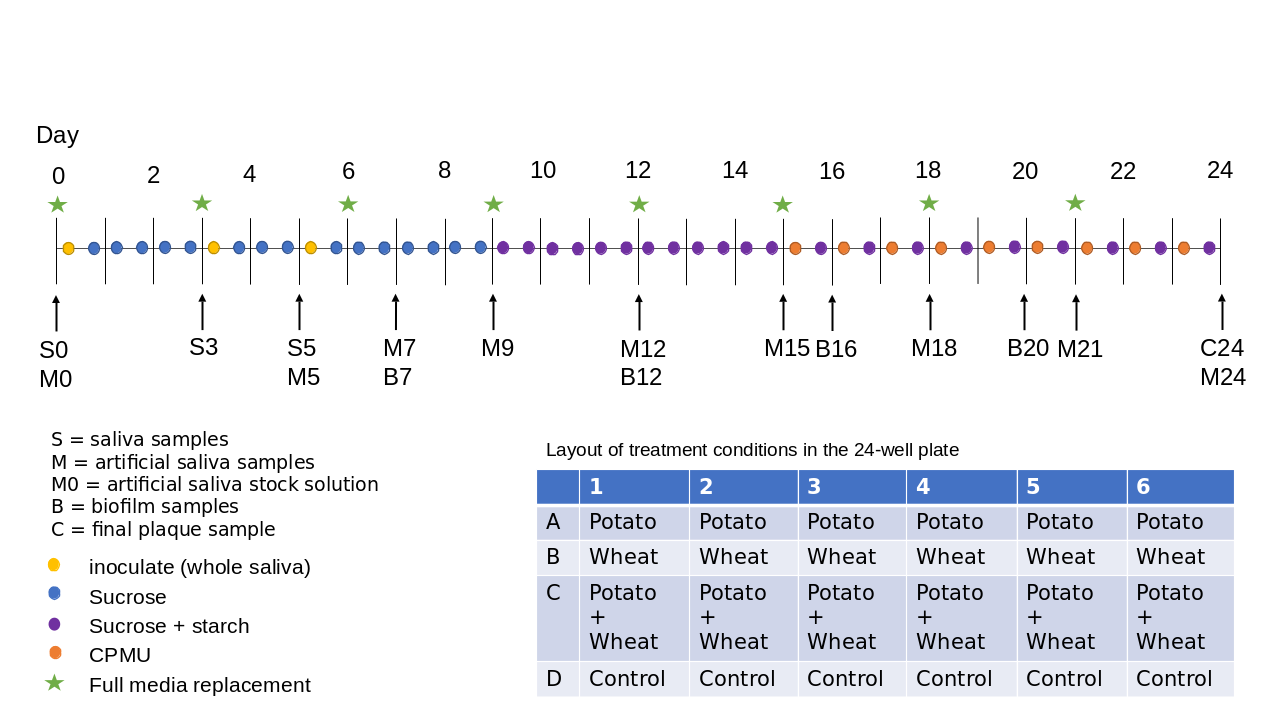
\includegraphics{figures/Exp_protocol.png}

}

\caption{\label{fig-protocol}Overview of the protocol for biofilm
growth. The samples for metagenomic analysis were grown in a separate
experimental plate than the FTIR samples under the same experimental
conditions. Biofilm (B) and calculus (C) samples were used for FTIR
spectroscopy, and saliva (S) and artificial saliva (M) samples were used
for metagenomic analysis.}

\end{figure}

To determine the composition of microbial communities, we sampled the
medium from the biofilm wells over the course of the experiment and
sequenced the DNA to identify species that are present in the model, and
assess whether these mimic natural oral communities. During a separate
experimental run, under the same conditions, we directly sampled the
biofilms on multiple days and determined the mineral composition using
FTIR, and compared the spectra to those of natural dental calculus, both
modern and archaeological. Samples were taken from both controls and
starch treatments, but differences between these samples were not
explored in this study.

\hypertarget{biofilm-growth}{%
\subsection{Biofilm growth}\label{biofilm-growth}}

We employ a multispecies oral biofilm model following a modified
protocol from Sissons and colleagues (1991) and Shellis (1978). The
setup comprises a polypropylene 24 deepwell PCR plate (KingFisher
97003510) with a lid containing 24 pegs (substrata), which are
autoclaved at 120\(^{\circ}\)C, 1 bar overpressure, for 20 mins.

The artificial saliva (hereafter referred to as medium) is a modified
version of the basal medium mucin (BMM) described by Sissons and
colleagues (1991). It is a complex medium containing 2.5 g/l partially
purified mucin from porcine stomach (Type III, Sigma M1778), 5 g/l
trypticase peptone (Roth 2363.1), 10 g/l proteose peptone (Oxoid
LP0085), 5 g/l yeast extract (BD 211921), 2.5 g/l KCl, 0.35 g/l NaCl,
1.8 mmol/l CaCl\textsubscript{2}, 5.2 mmol/l
Na\textsubscript{2}HPO\textsubscript{4} (Sissons et al., 1991), 6.4
mmol/l NaHCO\textsubscript{3} (Shellis, 1978), 2.5 mg/l haemin. This is
subsequently adjusted to pH 7 with NaOH pellets and stirring, autoclaved
(15 min, 120\(^{\circ}\)C, 1 bar overpressure), and supplemented with
5.8 (mu)mol/l menadione, 5 mmol/l urea, and 1 mmol/l arginine (Sissons
et al., 1991).

Fresh whole saliva (WS) for inoculation was provided by a 31-year-old
male donor with no history of caries, who abstained from oral hygiene
for 24 hours, and no food was consumed two hours prior to donation. No
antibiotics were taken up to six months prior to donation. Saliva was
stimulated by chewing on parafilm, then filtered through a
bleach-sterilised nylon cloth to remove particulates. Substrata were
inoculated with 1 ml/well of a two-fold dilution of WS in sterilised
20\% glycerine for four hours at 36\(^{\circ}\)C, to allow attachment of
the salivary pellicle and plaque-forming bacteria. After initial
inoculation, the substrata were transferred to a new plate containing 1
ml/well medium and incubated at 36\(^{\circ}\)C, with gentle motion at
30 rpm. The inoculation process was repeated on days 3 and 5 by
transferring the samples to a new plate with inoculate. Medium was
partially refreshed once per day, by topping up the wells to the
original volume with more medium, and fully refreshed every three days,
throughout the experiment, by transferring the substrata to a new plate
containing medium. To feed the bacteria, the substrata were transferred
to a new plate, containing 5\% (w/v) sucrose, for six minutes twice
daily, except on inoculation days (days 0, 3, and 5), where the samples
only received one sucrose treatment after inoculation.

On day 9, starch treatments were introduced, replacing sucrose
treatments (except for control sample). As with the sucrose treatments,
starch treatments occurred twice per day for six minutes, and involved
transferring the substrata to a new plate containing a 0.25\% (w/v)
starch from potato (Roth 9441.1) solution, a 0.25\% (w/v) starch from
wheat (Sigma S5127) solution, and a 0.5\% (w/v) mixture of equal
concentrations (w/v) wheat and potato. All starch solutions were created
in a 5\% (w/v) sucrose solution. Before transferring biofilm samples to
the starch treatments, the starch plates were agitated to keep the
starches in suspension in the solutions, and during treatments, the rpm
was increased to 60. The purpose of starch treatments was to explore the
incorporation of starch granules into the model calculus. Starch
treatments were initiated on day 9 (Figure~\ref{fig-protocol}) to avoid
starch granule counts being affected by \(\alpha\)-amylase hydrolysis
from the inoculation saliva. An \(\alpha\)-amylase assay conducted on
samples from days 3, 6, 8, 9, 10, 12, and 14 also showed that there was
no host salivary \(\alpha\)-amylase activity in the system. The results
of the starch incorporation and \(\alpha\)-amylase activity assay have
been reported in a separate article (Bartholdy \& Henry, 2022).

After 15 days, mineralisation was encouraged with a calcium phosphate
monofluorophosphate urea (CPMU) solution containing 20 mmol/l
CaCl\textsubscript{2}, 12 mmol/l
NaH\textsubscript{2}PO\textsubscript{4}, 5 mmol/l
Na\textsubscript{2}PO\textsubscript{3}F, 500 mmol/l urea (Pearce \&
Sissons, 1987; Sissons et al., 1991), and 0.04 g/l MgCl. The substrata
were submerged in 1 ml/well CPMU five times daily, every two hours, for
six minutes, at 30 rpm. During the mineralisation period, starch
treatments were reduced to once per day, two hours after the last CPMU
treatment. This cycle was repeated for 10 days until the end of the
experiment on day 24 (Figure~\ref{fig-protocol}). More detailed
protocols are available at
\url{https://dx.doi.org/10.17504/protocols.io.dm6gpj9rdgzp/v1}.

All laboratory work was conducted in sterile conditions under a laminar
flow hood to prevent starch and bacterial contamination. Starch-free
control samples that were only fed sucrose were included to detect
starch contamination.

\hypertarget{metagenomics}{%
\subsection{Metagenomics}\label{metagenomics}}

\hypertarget{tbl-dna-samples}{}
\begin{longtable}[]{@{}lrr@{}}
\caption{\label{tbl-dna-samples}Number of samples taken during the
experiment, separated by sampling day and sample type.}\tabularnewline
\toprule()
Sample type & Sampling day & n \\
\midrule()
\endfirsthead
\toprule()
Sample type & Sampling day & n \\
\midrule()
\endhead
saliva & 0 & 1 \\
saliva & 3 & 1 \\
saliva & 5 & 1 \\
medium & 5 & 2 \\
medium & 7 & 2 \\
medium & 9 & 2 \\
medium & 12 & 2 \\
medium & 15 & 2 \\
medium & 18 & 2 \\
medium & 21 & 2 \\
medium & 24 & 2 \\
model\_calculus & 24 & 16 \\
\bottomrule()
\end{longtable}

A total of 35 samples were taken during the experiment from the donated
saliva, artificial saliva, and from the biofilm end-product on day 24
(Table~\ref{tbl-dna-samples}). DNA extraction was performed at the Max
Planck Institute for the Science of Human History (Jena, Germany), using
the DNeasy PowerSoil Kit from QIAGEN. C2 inhibitor removal step skipped,
going directly to C3 step.

The DNA was sheared to 500bp through sonication with a Covaris M220
Focused-ultrasonicator. Double-stranded libraries were prepared (Aron et
al., 2020) and dual indexed (Stahl et al., 2019), with the indexing
protocol being adapted for longer DNA fragments. Briefly, the
modifications consisted of adding 3 μl of DMSO to the indexing reaction,
and extending the amplification cycles to 95\(^{\circ}\)C for 60 s,
58\(^{\circ}\)C for 60 s, and 72\(^{\circ}\)C for 90 s. The libraries
were paired-end sequenced on a NextSeq 500 to 150bp, and demultiplexed
by an in-house script.

\hypertarget{preprocessing}{%
\subsubsection{Preprocessing}\label{preprocessing}}

The raw DNA reads were preprocessed using the nf-core/eager, v2.4.4
pipeline (Fellows Yates et al., 2020). The pipeline included adapter
removal and read merging using AdapterRemoval, v2.3.2 (Schubert et al.,
2016). Merged reads were mapped to the human reference genome (GRCh38)
using BWA, v0.7.17-r1188 (Li \& Durbin, 2009) (-n 0.01; -l 32), and
unmapped reads were extracted using Samtools, v1.12. The final step of
the pipeline, metagenomic classification, was conducted in kraken,
v2.1.2 (Wood et al., 2019) using the Standard 60GB database
(\url{https://genome-idx.s3.amazonaws.com/kraken/k2_standard_20220926.tar.gz}).

Environmental reference samples were downloaded directly from ENA and
from NCBI using the SRA Toolkit. Oral reference samples were downloaded
from the Human Metagenome Project (HMP), and modern calculus samples
from Velsko et al. (2017). From the HMP data, only paired reads were
processed, singletons were removed. \emph{In vitro} biofilm model
samples from Edlund et al. (2018) were used as a reference. Links to the
specific sequences are included in the metadata. Human-filtered reads
produced in this study were uploaded to ENA under accession number
PRJEB61886.

\hypertarget{authentication}{%
\subsubsection{Authentication}\label{authentication}}

Species with lower than 0.001\% relative abundance across all samples
were removed from the species table. SourceTracker2 (Knights et al.,
2011) was used to estimate source composition of the abundance-filtered
oral biofilm model samples using a Bayesian framework, and samples
falling below 70\% oral source were removed from downstream analyses.
Well-preserved abundance-filtered samples were compared to oral and
environmental controls to detect potential external contamination. The R
package decontam v1.20.0 (Davis et al., 2018) was used to identify
potential contaminants in the abundance-filtered table using DNA
concentrations with a probability threshold of 0.95 and negative
controls with a probability threshold of 0.05. Putative contaminant
species were filtered out of the OTU tables for all downstream analyses.

\hypertarget{community-composition}{%
\subsubsection{Community composition}\label{community-composition}}

Relative abundances of communities were calculated at the species- and
genus-level, as recommended for compositional data (Gloor et al., 2017).
Shannon index and Pileou's evenness index were calculated on
species-level OTU tables of all model and oral reference samples using
the vegan v2.6.4 R package (Oksanen et al., 2022). Shannon index was
calculated for all experimental samples to see if there is an overall
loss or gain in diversity and richness across the experiment. Sparse
principal component analysis (sPCA) was performed on model biofilm
samples to assess differences in microbial composition between samples
within the experiment, and a separate sPCA analysis was performed on
model calculus and oral reference samples. The sPCA analysis was
conducted using the mixOmics v 6.24.0 R package (Rohart et al., 2017).

The core microbiome was calculated by taking the mean genus-level
relative abundance within each sample type for model calculus, modern
reference calculus, sub- and supragingival plaque. Genera present at
lower than 5\% relative abundance were grouped into the category
`other'. Information on the oxygen tolerance of bacterial species was
downloaded from BacDive (Reimer et al., 2022) and all variations of the
major categories anaerobe, facultative anaerobe, and aerobe were
combined into the appropriate major category. At the time of writing,
55.7\% species were missing aerotolerance values. This was mitigated by
aggregating genus-level tolerances to species with missing values, and
may have some errors (although unlikely to make any significant
difference).

\hypertarget{differential-abundance}{%
\subsubsection{Differential abundance}\label{differential-abundance}}

Differential abundance of species was calculated using the Analysis of
Compositions of Microbiomes with Bias Correction (ANCOM-BC) method from
the ANCOMBC R package v2.2.0 (Lin \& Peddada, 2020), with a
species-level OTU table as input. Results are presented as the log fold
change of species between paired sample types with 95\% confidence
intervals. P-values are adjusted using the false discovery rate (FDR)
method. Samples are grouped by sample type (i.e.~saliva, plaque, modern
calculus, model calculus). To supplement the sPCA analyses, we
visualised the log-fold change of the top 30 species in each of
principal components 1 and 2, allowing us to see which species are
enriched in the different samples and causing clustering in the sPCA.

\hypertarget{ftir}{%
\subsection{FTIR}\label{ftir}}

To determine the mineral composition and level of crystallisation of the
model dental calculus samples, we used Fourier Transform Infrared (FTIR)
spectroscopy. We compared the spectra of model dental calculus with
spectra of archaeological and modern dental calculus and used a built-in
Omnic search library for mineral identification (Mentzer et al., 2014;
Weiner, 2010a). The archaeological dental calculus was sampled from an
isolated permanent tooth from Middenbeemster, a rural, 19th century
Dutch site (Lemmers et al., 2013). Samples were analysed at the
Laboratory for Sedimentary Archaeology, Haifa University. The analysis
was conducted with a Thermo Scientific Nicolet is5 spectrometer in
transmission, at 4 cm\(^{-1}\) resolution, with an average of 32 scans
between 4000 and 400 cm\(^{-1}\) wavenumbers.

\hypertarget{tbl-ftir-byoc}{}
\begin{longtable}[]{@{}lrrr@{}}
\caption{\label{tbl-ftir-byoc}Summary of samples used in FTIR analysis,
including type of sample, sampling day, number of samples (n), and mean
weight in mg.}\tabularnewline
\toprule()
Sample type & Sampling day & n & Weight (mg) \\
\midrule()
\endfirsthead
\toprule()
Sample type & Sampling day & n & Weight (mg) \\
\midrule()
\endhead
biofilm & 7 & 2 & 0.79 \\
biofilm & 12 & 3 & 1.01 \\
biofilm & 16 & 7 & 2.00 \\
biofilm & 20 & 6 & 3.50 \\
model\_calculus & 24 & 8 & 3.87 \\
\bottomrule()
\end{longtable}

Analysis was conducted on 26 model calculus samples from days 7, 12, 16,
20, and 24 (Table~\ref{tbl-ftir-byoc}). Some samples from the same
sampling day had to be combined to provide enough material for analysis.
Samples analysed with FTIR were grown during a separate experimental run
from the samples sequenced for DNA, but following the same setup and
protocol (as described above). Samples were analysed following the
method presented in Asscher, Regev, et al. (2011) and Asscher, Weiner,
et al. (2011). A few \(\mu\)g of each sample were repeatedly ground
together with KBr and pressed in a 7 mm die under two tons of pressure
using a Specac mini-pellet press (Specac Ltd., GS01152). Repeated
measurements of the splitting factor (SF) of the absorbance bands at 605
and 567 cm−1 wavenumbers were taken after each grind, and a grind curve
was produced following Asscher, Regev, et al. (2011) to try and detect
changes in the hydroxyapatite crystallinity over time. Samples were
ground and analysed up to six times (sample suffix a-f) for the grinding
curve. Grinding curves were prepared for samples from days 16, 20, and
24. No grind curves were produced for samples from days 7 and 12. These
were largely composed of organics and proteins, and did not form enough
mineral (hydroxyapatite) for analysis. The splitting factor of carbonate
hydroxyapatite was calculated using a macro script, following Weiner \&
Bar-Yosef (1990). The calculation involves dividing the sum of the
height of the absorptions at 603 cm\(^{-1}\) and 567 cm\(^{-1}\) by the
height of the valley between them. Following Asscher, Regev, et al.
(2011) and Asscher, Weiner, et al. (2011), we plotted the splitting
factor against the full width at half maximum (FWHM) of the main
absorption at 1035-1043 cm\(^{-1}\) to explore crystallinity (crystal
size) and the order and disorder of hydroxyapatite. We then compared our
grinding curve slopes and FWHM to the ones produced by Asscher, Weiner,
et al. (2011). Asscher, Weiner, et al. (2011) and Asscher, Regev, et al.
(2011) demonstrated that while the decrease in FWHM of each grinding in
the curve reflects a decrease in particle size due to grinding, the
location of the curves within a plot of the FWHM against the splitting
factor expresses the disorder effect. Thus the curves with steeper
slopes, higher splitting factor, and lower FWHM represent lower levels
of disorder in the mineral (Figure 2 in Asscher, Weiner, et al., 2011).

\hypertarget{statistics}{%
\subsection{Statistics}\label{statistics}}

Statistical analysis was conducted in R version 4.3.0 (2023-04-21)
(Already Tomorrow) (R Core Team, 2020). Data cleaning and wrangling
performed with packages from tidyverse (Hadley Wickham et al., 2019).
Plots were created using ggplot2 v3.4.2 (H. Wickham, 2016).

\hypertarget{results}{%
\section{Results}\label{results}}

\hypertarget{metagenomic-analysis}{%
\subsection{Metagenomic analysis}\label{metagenomic-analysis}}

\hypertarget{sample-authentication}{%
\subsubsection{Sample authentication}\label{sample-authentication}}

To determine the extent of contamination in our samples, we performed a
source-tracking analysis using SourceTracker2 (Knights et al., 2011).
Results suggest that the majority of taxa across samples have an oral
microbial signature, and therefore our samples are minimally affected by
external contamination (Figure S1). We compared SourceTracker2 results
to a database of oral taxa from the cuperdec v1.1.0 R package (Fellows
Yates et al., 2021) to prevent removal of samples where oral taxa were
assigned to a non-oral source (Figure S2), as some taxa with a signature
from multiple sources are often classified as ``Unknown'' (Velsko et
al., 2019). We included several oral sources, which may increase the
risk of this occurring. Samples containing a large proportion
(\textgreater70\%) of environmental contamination were removed. The
removed samples were predominantly medium samples from later in the
experiment, and a few model calculus samples. After contaminated samples
were removed, suspected contaminant-species were removed from the
remaining samples using the decontam R package (Davis et al., 2018).
After contamination removal, samples consisted of between 88 and 284
species with a mean of 182.

\hypertarget{decrease-in-community-diversity-across-experiment}{%
\subsubsection{Decrease in community diversity across
experiment}\label{decrease-in-community-diversity-across-experiment}}

\begin{figure}

{\centering 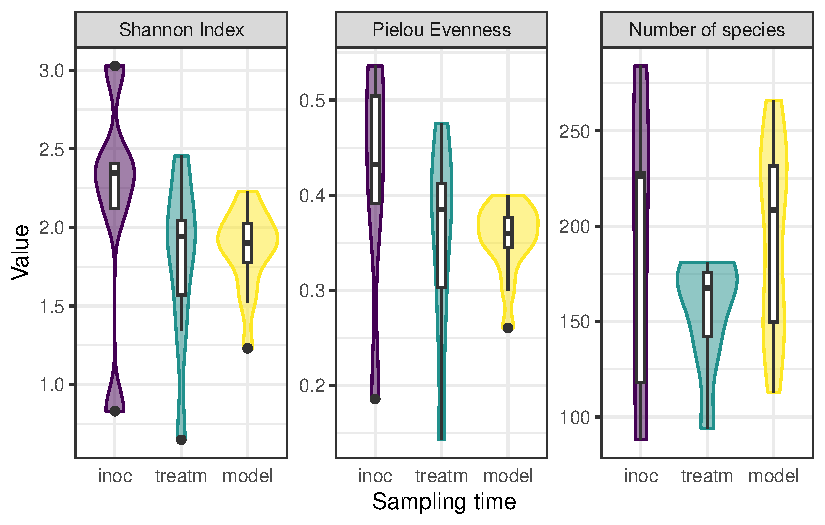
\includegraphics{index_files/figure-pdf/fig-diversity-byoc-1.pdf}

}

\caption{\label{fig-diversity-byoc}Plot of Pielou Evenness Index, number
of species, and Shannon Index across experiment samples grouped by
sampling time. inoc = samples from days 0-5; treatm = samples from days
6-23; model = model calculus samples from day 24.}

\end{figure}

To monitor the development of microbial communities over the course of
the experiment, we used the Shannon Index to assess the species
diversity and richness at various stages of our protocol. Samples were
grouped into sampling categories due to low sample sizes on sampling
days (inoc = days 0, 3, 5; treatm = days 7, 9, 12, 15; model = day 24).
There was a slight decrease in mean Shannon Index between inoculation
(mean {[}M{]} = 2.15 \(\pm\) 0.808) and treatment samples (M = 1.78
\(\pm\) 0.568), followed by a slight increase to model calculus samples
(M = 1.86 \(\pm\) 0.261), as well as a decrease in variance within
samples types (Figure~\ref{fig-diversity-byoc}). The Pielou Evenness
Index showed a similar pattern (M = 0.41 \(\pm\) 0.138; M = 0.351
\(\pm\) 0.108; M = 0.354 \(\pm\) 0.0379), while number of species
increased between the treatment period and the final model calculus (M =
189 \(\pm\) 82.4; M = 155 \(\pm\) 29.8; M = 194 \(\pm\) 49.2).

\hypertarget{medium-and-model-calculus-samples-are-distinct-from-the-inoculate}{%
\subsubsection{Medium and model calculus samples are distinct from the
inoculate}\label{medium-and-model-calculus-samples-are-distinct-from-the-inoculate}}

\begin{figure}

{\centering 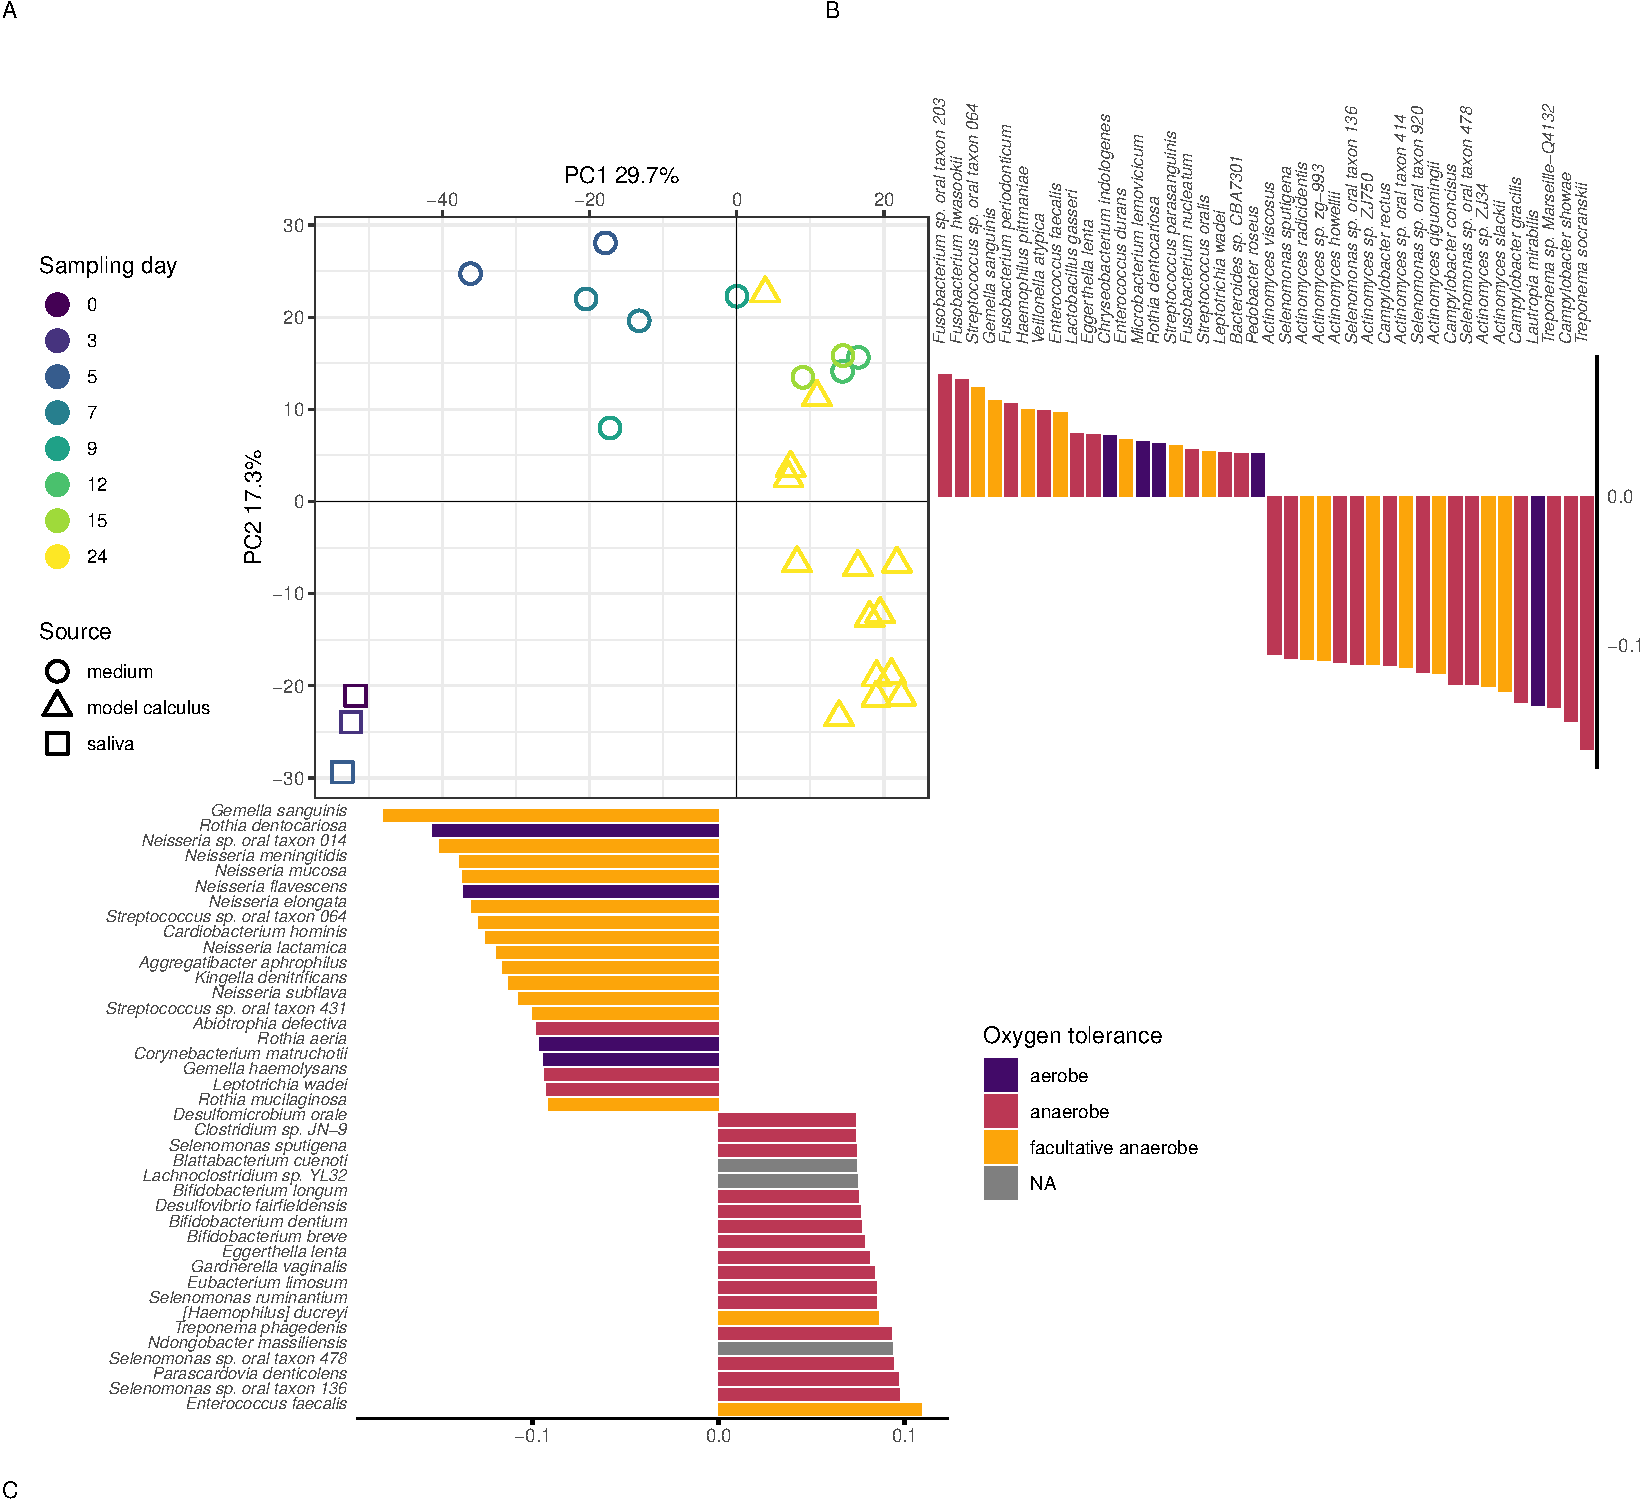
\includegraphics{index_files/figure-pdf/fig-spca-byoc-1.pdf}

}

\caption{\label{fig-spca-byoc}sPCA on species-level counts and oxygen
tolerance in samples from this study only. Figure shows the main sPCA
plot (A), species loadings on PC2 (B), and species loadings on PC1 (C).}

\end{figure}

We next examined whether there is a change in the species composition
over time in our samples by assessing the beta-diversity in a PCA. The
species profiles of the saliva inoculate used in our experiment were
distinct from both medium and model calculus samples. Most of the
separation of saliva from model calculus is on PC1 of the sPCA, where
most of the positive sample loadings are driven by anaerobic species
(model calculus), especially \emph{Selenomonas} spp, and negative
loadings are predominantly facultative anaerobes and some aerobes, such
as \emph{Rothia} and \emph{Neisseria} spp (saliva). Medium and saliva
are separated mostly on PC2, with medium samples located between saliva
and model calculus samples. Model calculus samples also cluster
separately from the medium samples on PC2, with some overlap between the
more mature medium samples and model calculus. Most of the negative
loadings separating saliva and model calculus from medium samples are
dominated by \emph{Actinomyces} spp., while positive species loadings
are more diverse, and seemingly unrelated to aerotolerance
(Figure~\ref{fig-spca-byoc}).

\begin{figure}

{\centering 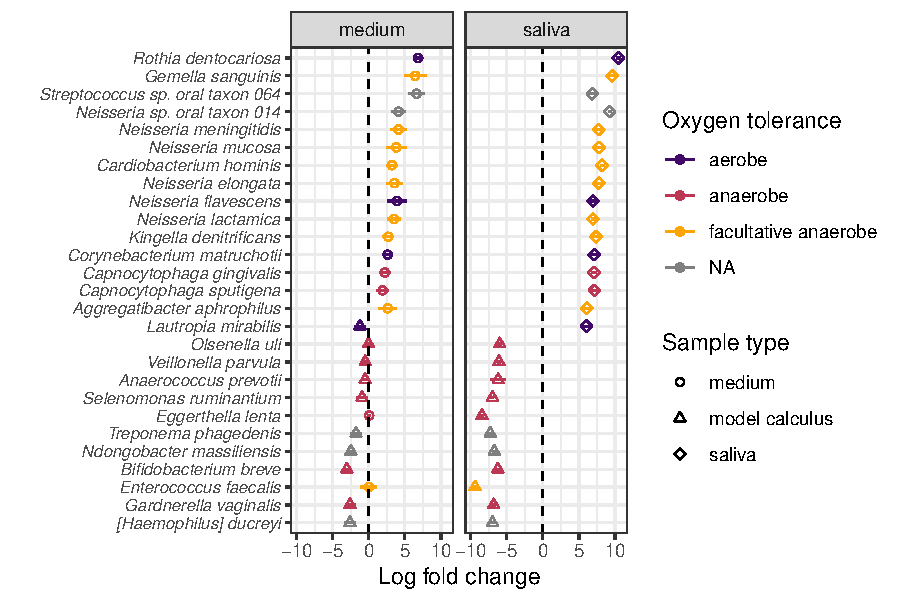
\includegraphics{index_files/figure-pdf/fig-diffabund-byoc-1.pdf}

}

\caption{\label{fig-diffabund-byoc}Log-fold changes between sample
types. Circles are species enriched in the model calculus, squares are
enriched in saliva, and triangles in medium. Lines are standard error.
Plot shows the top 30 absolute log-fold changes between model calculus
and saliva.}

\end{figure}

We determined whether there are speices that are differentially abundant
between our sample types using the ANCOMBC R package (Lin \& Peddada,
2020), giving us an idea of how the biofilm develops under our
experimental conditions. Species enriched in saliva compared to model
calculus are largely aerobic or facultatively anaerobic, while species
enriched in model calculus compared to saliva are mainly anaerobes. The
differences between saliva and calculus are more pronounced than between
medium and model calculus, which is expected
(Figure~\ref{fig-diffabund-byoc}).

\hypertarget{lower-diversity-in-artificial-samples-than-oral-references}{%
\subsubsection{Lower diversity in artificial samples than oral
references}\label{lower-diversity-in-artificial-samples-than-oral-references}}

\begin{figure}

{\centering 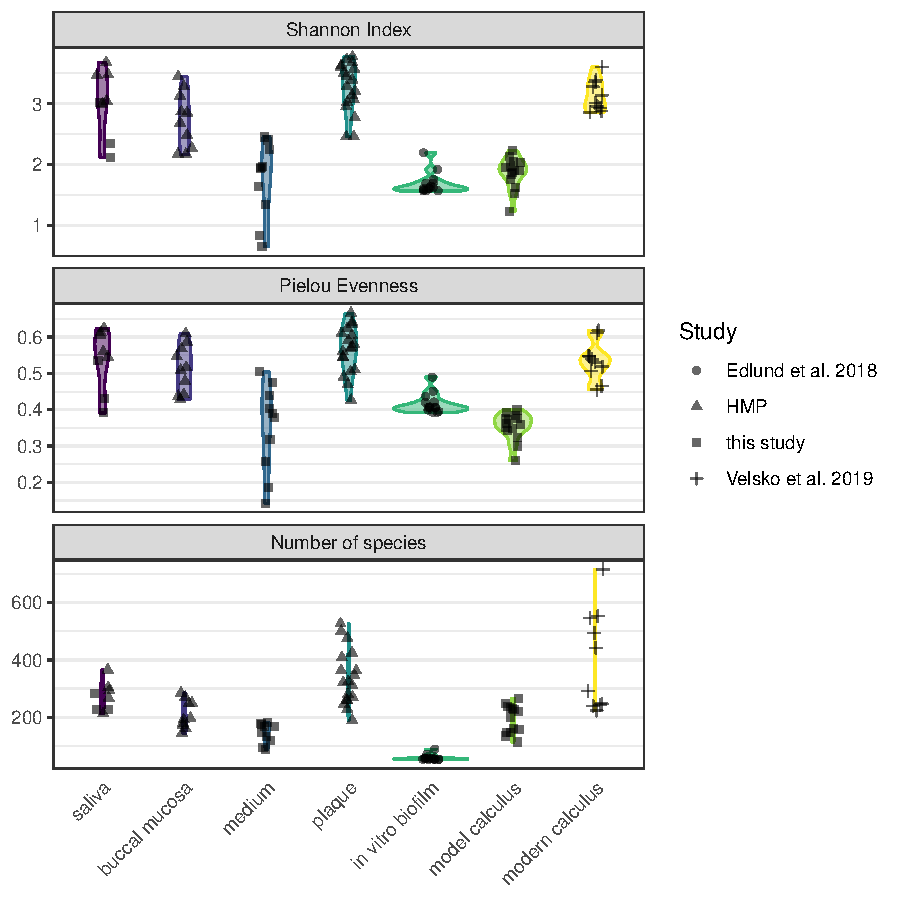
\includegraphics{index_files/figure-pdf/fig-shannon-compar-1.pdf}

}

\caption{\label{fig-shannon-compar}Shannon Index for model calculus and
medium samples, as well as oral reference samples and comparative
\emph{in vitro} study.}

\end{figure}

We used the Shannon Index to compare alpha-diversity in our model to
oral reference samples. The mean Shannon Index of model
samples---medium, model calculus, reference \emph{in vitro} biofilm (M =
1.74 \(\pm\) 0.627; M = 1.86 \(\pm\) 0.261; M = 1.69 \(\pm\) 0.173,
respectively) were consistently lower than the means of oral reference
samples---mucosa, modern reference dental calculus, saliva, and
subgingival and subgingival plaque (M = 2.74 ± 0.461; M = 3.14 ± 0.255;
M = 3.02 ± 0.548; M = 3.53 ± 0.241; M = 3.04 ± 0.391). The Pielou
species evenness index has a similar distribution, although the
comparative biofilm samples have a higher mean than biofilm samples from
this study. Saliva inoculate samples from this study (M = 2.5 \(\pm\)
0.472 have a lower mean Shannon index than reference samples (M = 3.33
\(\pm\) 0.297), which may have contributed to the lower alpha-diversity
in model samples compared to reference samples.

\hypertarget{model-calculus-is-distinct-from-dental-calculus-and-other-oral-samples}{%
\subsubsection{Model calculus is distinct from dental calculus and other
oral
samples}\label{model-calculus-is-distinct-from-dental-calculus-and-other-oral-samples}}

\begin{figure}

{\centering 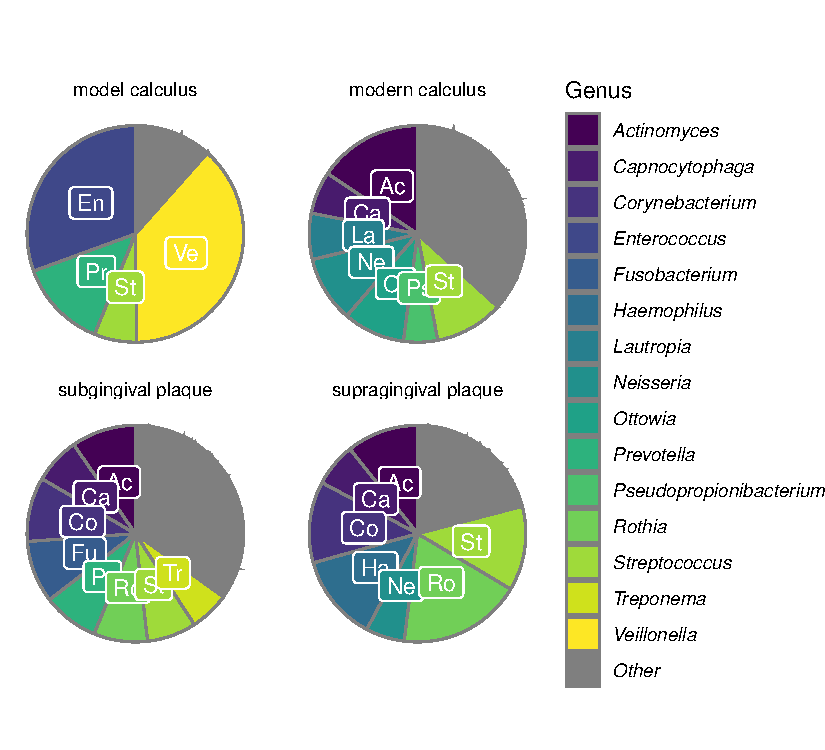
\includegraphics{index_files/figure-pdf/fig-core-genera-1.pdf}

}

\caption{\label{fig-core-genera}Core genera within the different types
of samples represented as mean relative abundances at the genus level.
Other = other genera present in lower than 5\% relative abundance.}

\end{figure}

We calculated the mean relative abundances at the genus in each sample
to compare the core genera of model calculus with oral reference
samples, with the most common genera (\textgreater5\% relative
abundance) shown in Figure~\ref{fig-core-genera}. The main overlap
between the model calculus and oral reference samples is the high
relative abundance of \emph{Streptococcus}. Model calculus consists
mostly of \emph{Enterococcus} and \emph{Veillonella} spp., despite both
having low abundance in donor saliva, while oral reference samples are
more diverse (Figure~\ref{fig-core-genera}), which is consistent with
the alpha diversity calculations.

\begin{figure}

{\centering 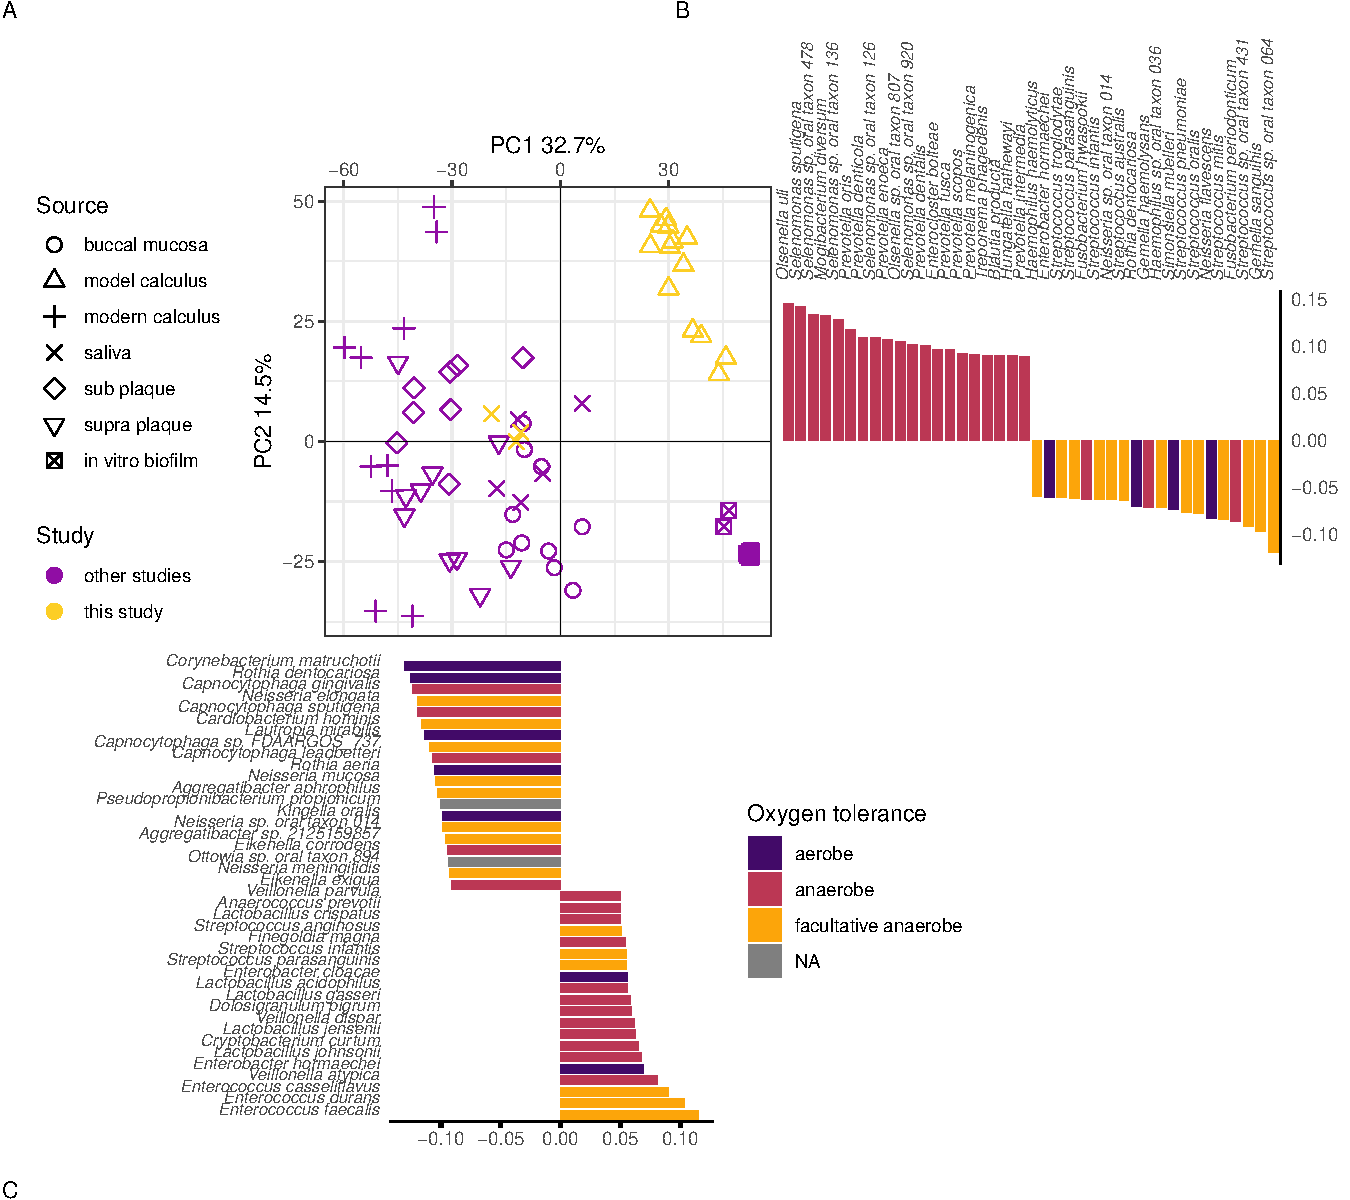
\includegraphics{index_files/figure-pdf/fig-spca-compar-1.pdf}

}

\caption{\label{fig-spca-compar}sPCA on species-level counts from model
calculus and reference samples. Figure shows (A) the main sPCA plot, (B)
the species loadings from PC2, and (C) species loadings on PC1.}

\end{figure}

To directly compare the beta-diversity of our model calculus with oral
reference samples, including modern dental calculus, we used an sPCA
including only our model calculus and reference samples. Model calculus
samples are distinct from both the oral reference samples and the
biofilm model reference samples. They are separated from oral reference
samples mainly on PC1, and from biofilm model reference samples (and, to
some extent, oral samples) on PC2. The highest negative contributions
are a mix of all types of aerotolerance, while the positive
contributions are mostly (facultative) anaerobes, with
\emph{Enterococcus} spp. as the top three positive contributors to PC1.
Top negative contributors are \emph{Capnocytophaga} spp as well as the
aerobes \emph{Corynebacterium matruchotii} and \emph{Rothia
dentocariosa}. The top positive contributors to PC2 are all anaerobes,
mainly from the genus \emph{Selenomonas}. Top negative contributors to
PC2 are a mix of aerotolerances, with many \emph{Streptococcus} spp.

\begin{figure}

{\centering 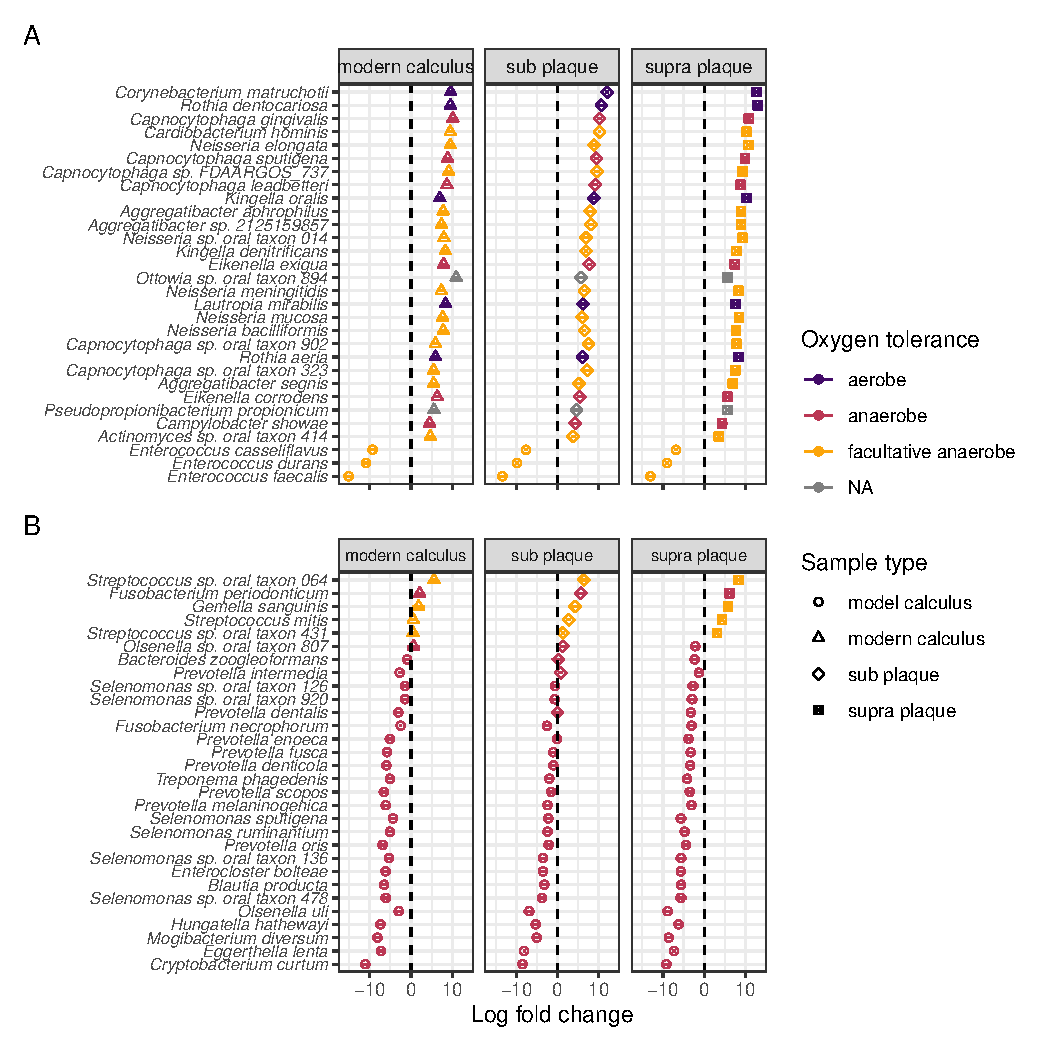
\includegraphics{index_files/figure-pdf/fig-diffabund-comp-1.pdf}

}

\caption{\label{fig-diffabund-comp}Log-fold changes between sample
types. Circles are species enriched in the model calculus, triangles in
modern calculus, diamonds are enriched in subgingival plaque, and
squares in supragingival plaque. Plot shows the top 30 loadings
(absolute value) in PC1 (A) and PC2 (B) between model calculus and other
sample types, ordered by decreasing log-fold change. Bars represent
standard error.}

\end{figure}

To investigate which species are enriched in different sample types, and
compare the final product of our model with naturally occurring plaque
and calculus samples, we performed differential abundance analysis on
our model calculus samples, modern dental calculus, and sub- and
supragingival plaque. Based on the differential abundance analysis the
main differences between model calculus and oral reference samples, when
looking at the top 30 contributors to PC1, are that the oral reference
samples are enriched with species with a diverse oxygen tolerance from a
wide range of genera, while the model calculus is enriched with
\emph{Enterococcus} spp. The largest differences occur in
\emph{Corynebacterium matruchotii}, \emph{Rothia dentocariosa}, and
\emph{Capnocytophaga gingivalis} (Figure~\ref{fig-diffabund-comp}A).
This is echoed when looking at the top 30 contributors to PC2, where
most of the species are enriched in model calculus, all of which are
anaerobes, and the largest differences occurring in
\emph{Cryptobacterium curtum}, \emph{Eggerthella lenta}, and
\emph{Mogibacterium diversum} (Figure~\ref{fig-diffabund-comp}B).

\hypertarget{samples-show-an-increased-mineralisation-over-the-course-of-the-experiment}{%
\subsection{Samples show an increased mineralisation over the course of
the
experiment}\label{samples-show-an-increased-mineralisation-over-the-course-of-the-experiment}}

Comparing the development of the model calculus to the reference
samples, it is evident that between days 7 and 24 there is a decrease of
the protein components and increase of the inorganic mineral carbonate
hydroxyapatite. The model calculus samples from the end of the
experiment are similar to both the modern and archaeological reference
samples. The main difference is a lower organic component in reference
samples seen as a reduced amide I peak at around 1637 compared to the
carbonate peak at around 1420, and an absence of amide II and III.
Further, there is a reduction in CH3 bands at 3000-2900 cm\(^{-1}\)
(Figure~\ref{fig-ftir-spectra}A-D).

Sample spectra from days 7 and 12 are characterised by a high content of
proteins as evident by the strong amide I absorbance band at 1650, a
less pronounced amide II band at 1545 cm\(^{-1}\), and the small amide
III band at 1237 cm\(^{-1}\). Related to the organic component of the
samples are also the three marked CH\textsubscript{3} and
CH\textsubscript{2} stretching vibrations at 2960, 2920, and 2850
cm\(^{-1}\) wavenumbers. The presence of mineral component is evident
from the presence of C--O\(^{2-}_3\) absorbance bands at 1450 and 1400
cm\(^{-1}\) wavenumbers typical of carbonates, and P--O\(^{3-}_4\)
absorbance band at 1080 and 1056 cm\(^{-1}\) which are related to
phosphate minerals. There is a large variation between the spectra,
possibly indicating different formation rates of the different
components in the samples (Figure~\ref{fig-ftir-spectra}A and B).

In spectra from days 16 to 24, the ratio of amides to
PO\textsubscript{4} has shifted, with the main peak shifting to the
PO\textsubscript{4} v\textsubscript{3} absorbance band at 1039--1040
cm\(^{-1}\), indicating that the main component of the samples is
carbonate hydroxyapatite. A well-defined PO\textsubscript{4} doublet at
600 and 560 is present. Small CO\(_3^{2-}\) asymmetric stretching at
1450 cm\(^{-1}\) and 1415 cm\(^{-1}\), and stretching vibrations at
875-870 cm\(^{-1}\) indicate that the carbonate minerals component is
also becoming more crystallised. There is a decreased variability
between the spectra, with most spectra exhibiting a higher
phosphate-to-protein/lipid ratio (Figure~\ref{fig-ftir-spectra}C and D).

\hypertarget{model-calculus-has-a-similar-mineral-composition-to-natural-calculus}{%
\subsection{Model calculus has a similar mineral composition to natural
calculus}\label{model-calculus-has-a-similar-mineral-composition-to-natural-calculus}}

To determine whether the model dental calculus is comparable to natural
dental calculus, both modern and archaeological dental calculus were
analysed with FTIR spectroscopy to ascertain their composition. The
archaeological and modern reference spectra are largely
indistinguishable and consist of a broad O--H absorbance band (3400
cm\(^{-1}\)) related to amid a and hydroxyl group, weak CH3 bands
(3000--2900 cm\(^{-1}\)), amide I band (1650 cm\(^{-1}\)) which is
related to the protein content, carbonate (1420, 1458-1450, 875-870
cm\(^{-1}\)), and phosphates (1036-1040, 602-4, 563-566 cm\(^{-1}\))
(Figure~\ref{fig-ftir-spectra}E) which, together with the hydroxyl and
the carbonate, can be identified as derived from carbonate
hydroxyapatite, the main mineral found in mature dental calculus
(Hayashizaki et al., 2008; Jin \& Yip, 2002).

\begin{figure}

{\centering 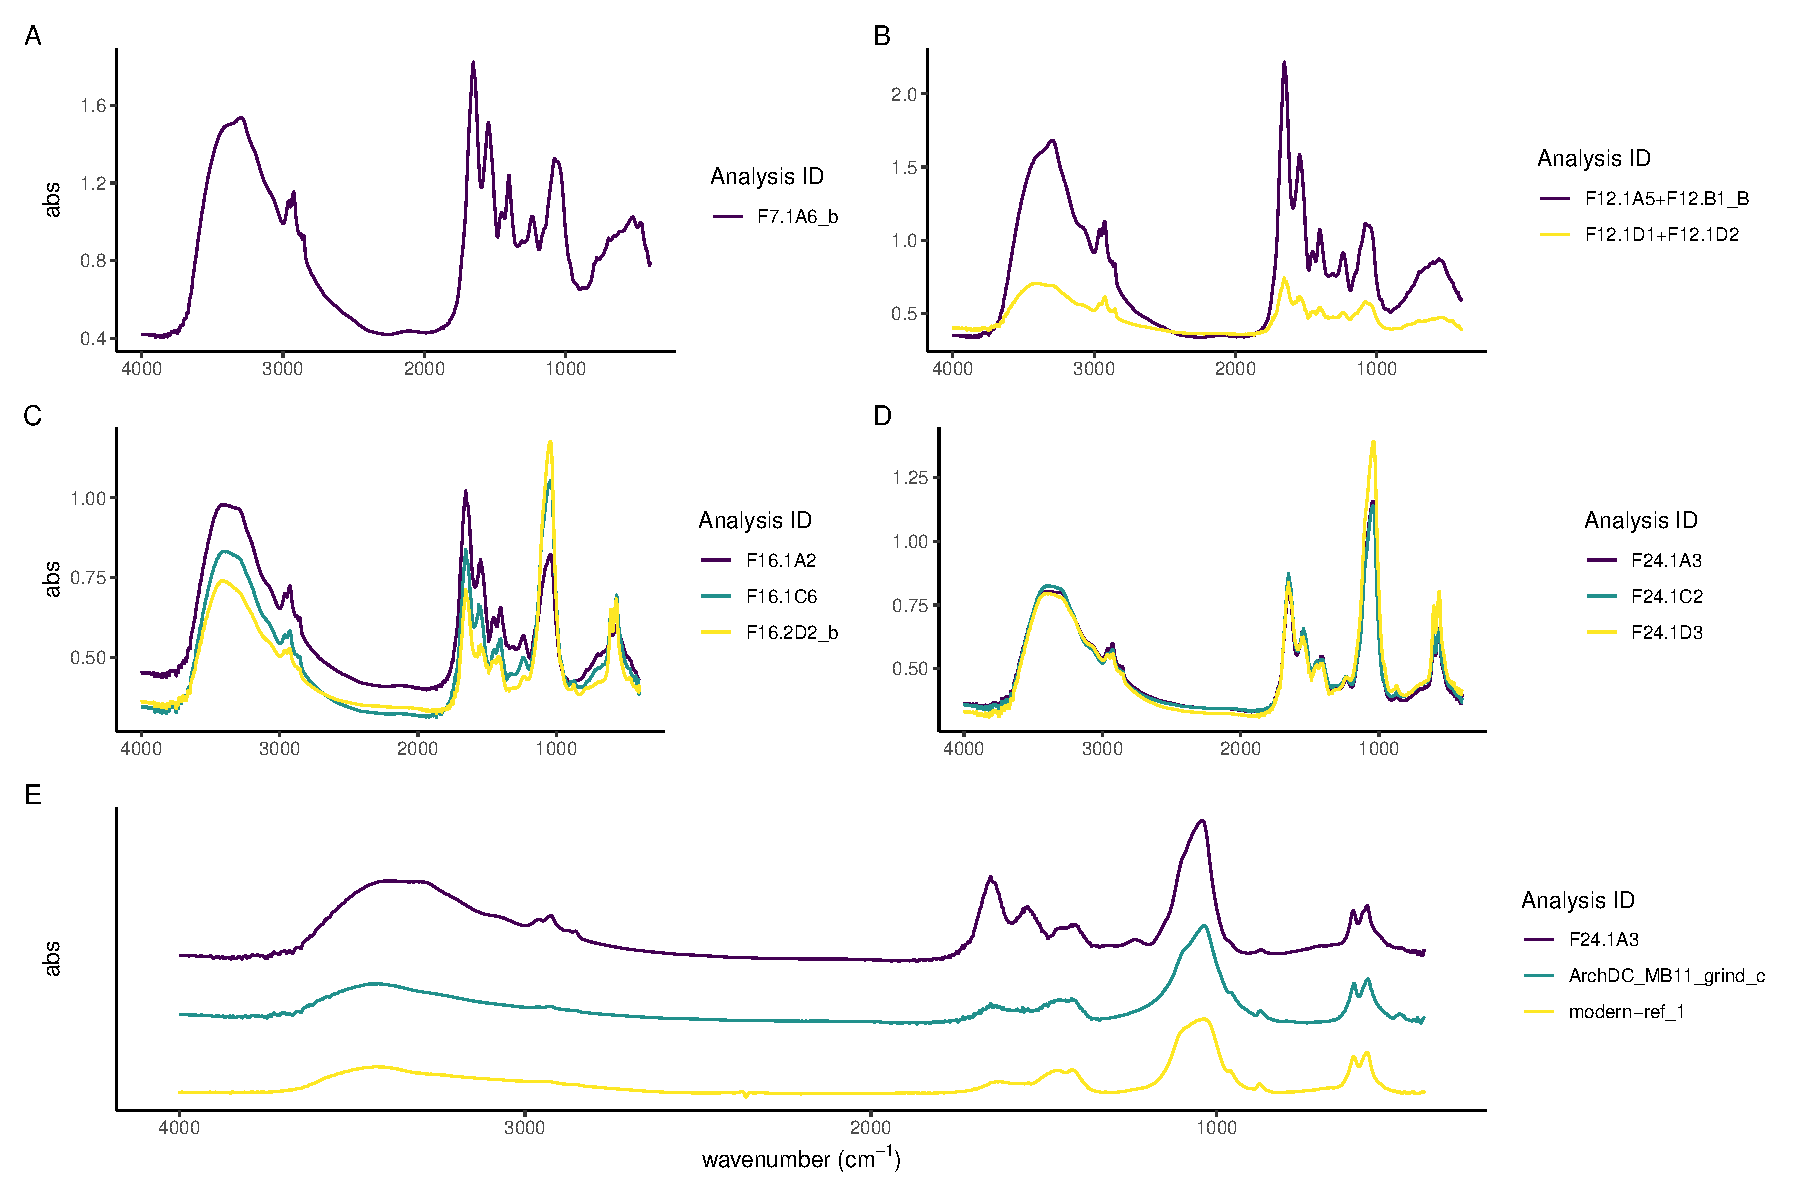
\includegraphics{index_files/figure-pdf/fig-ftir-spectra-1.pdf}

}

\caption{\label{fig-ftir-spectra}Select spectra from all experiment
sampling days; (A) day 7, (B) day 12, (C) day 16, and (D) day 24.
Absorbance bands in stretching mode around 3400 cm−1 typical of the
hydroxyl group. Analysis ID for model samples is constructed as: F{[}day
sampled{]}.{[}well sampled{]}\_{[}grind sample{]}.}

\end{figure}

\hypertarget{samples-show-similar-crystallinity-and-order-to-reference-calculus}{%
\subsection{Samples show similar crystallinity and order to reference
calculus}\label{samples-show-similar-crystallinity-and-order-to-reference-calculus}}

We determined the level of crystallinity and order of the carbonate
hydroxyapatite in our samples as an indication for its maturity by using
the grinding curves method presented by Asscher, Regev, et al. (2011)
and Asscher, Weiner, et al. (2011).\\
Samples were compared to published trendlines for archaeological and
modern enamel (Asscher, Regev, et al., 2011). We see no appreciable
differences between days 16, 20, and 24. The archaeological dental
calculus shows a slightly increased slope compared to model calculus
from the three sampling days used in the grind curve
(Figure~\ref{fig-grind-curve}), possibly indicating larger crystal size
due to more complete crystalisation. The steeper slope of enamel samples
is consistent with a more ordered structure in enamel compared to dental
calculus.

\begin{figure}

{\centering 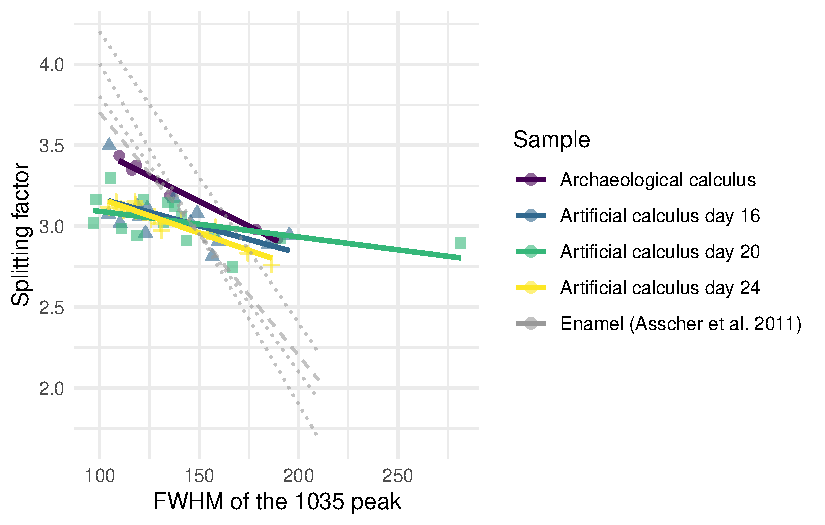
\includegraphics{index_files/figure-pdf/fig-grind-curve-1.pdf}

}

\caption{\label{fig-grind-curve}Grinding curves of our biofilm and model
calculus compared to published trendlines (dashed light grey lines) for
archaeological (dotted line) and modern (dashed line) enamel.}

\end{figure}

\hypertarget{discussion}{%
\section{Discussion}\label{discussion}}

In this study we present a calcifying oral biofilm model to produce
artificial dental calculus. Our proposed use of the model is to address
a variety of research questions related to dietary information extracted
from dental calculus, in both modern and archaeological samples. For
that to be feasible, the model needs to serve as a viable proxy to
dental calculus grown under natural conditions, i.e., in the human oral
cavity. It needs, as much as possible, to mimic the diversity and
complexity of the natural oral microbiome, while also offering control
over factors such as dietary input, growth conditions, and replicability
within and between experiments. Here, we assessed the viability of our
model as a proxy for dental calculus using metagenomic classification
and FTIR analysis to explore the bacterial and mineral composition, and
compare with oral reference samples.

\hypertarget{microbiome}{%
\subsection{Microbiome}\label{microbiome}}

There is a loss of diversity from inocula saliva to model calculus, and
when compared to oral reference samples, which is a common limitation in
biofilm models (Bjarnsholt et al., 2013; Edlund et al., 2013). The
donated saliva for the experiment had a lower diversity than the
reference saliva samples, and may have contributed to a lower diversity
in experimental samples. Consequently, there is also a lower diversity
and richness when compared to other modern oral reference samples,
including oral mucosa, saliva, plaque, and calculus. Samples of the
medium from early in the experiment have similar species profiles to the
donated saliva, but gradually diverge over the course of the experiment.
This may be caused by experimental setup not sufficiently mimicking the
oral environment, allowing different species to thrive that do not
normally thrive in the natural oral environment.

Model calculus has a lower alpha-diversity than modern reference
calculus and other oral reference samples, and clusters separately in
the sPCA analysis. Species within the genera \emph{Veillonella} and
\emph{Enterococcus} are the most abundant in model calculus samples,
followed by \emph{Streptococcus} and \emph{Prevotella}. Oral reference
samples have a relative abundance of streptococci similar to our model,
but a more diverse representation from other genera such as
\emph{Actinomyces}, \emph{Capnocytophaga}, and \emph{Fusobacterium}.
Especially \emph{Enterococcus} spp. seemed to thrive later in the
experiment, at the expense of fastidious early coloniser species like
\emph{Capnocytophaga} and \emph{Neisseria} spp., which require an
environment with at least 5\% carbon dioxide to thrive (Tønjum \& van
Putten, 2017). Our biofilm was grown under atmospheric carbon dioxide
levels outside of our control. While \emph{Enterococcus} spp. were
present (in low quantities) in donor saliva, they are also known
environmental contaminants, and we cannot exclude environmental
contamination as a possible source for these species in our model. The
separation of model calculus from other oral reference samples may also
be caused by a loss of diversity in aerotolerance. Of the dominant
species in the model, most are either anaerobes or facultative
anaerobes, predominantly Gram-negative \emph{Veillonella} and
\emph{Prevotella}, and Gram-positive \emph{Enterococcus}. Species within
predominantly aerobic genera, such as \emph{Neisseria}, \emph{Rothia},
and \emph{Ottowia}, are deficient in the model compared to the donated
saliva and other oral samples, suggesting a shift from a largely
aerotolerant profile to an anaerobic profile during the experiment.
While our model is not set up as an anaerobic system, the anaerobes seem
to have outcompeted aerobes and, to some extent, facultative anaerobes.
This is likely a result of communities of bacteria within the biofilm
creating favourable microenvironments facilitated by the protective
properties of the biofilm matrix (Edlund et al., 2018; Flemming et al.,
2016). \emph{Capnocytophaga} and \emph{Actinomyces} spp. are
predominantly (facultative) anaerobes, so their deficiency may be
attributed to, for example, nutrient availability or being out-competed
by other species.

Overall, the main causes of separation seem to be the abundance of
(facultative) anaerobes in the model compared to reference calculus, and
the overgrowth of \emph{Enterococcus} spp. \emph{E. faecalis}, \emph{E.
durans}, and \emph{E. casseliflavus}. This may be due to human
variation, as there can be large differences in the oral microbiome of
two individuals at the species level due to variations in age, sex, and
other demographic factors, as well as how and when saliva samples were
collected (Burcham et al., 2020; Nearing et al., 2020). It may also be a
problem in oral biofilm models in general, as the reference \emph{in
vitro} samples also have a high abundance of \emph{Enterococcus} spp.
Whether or not distinct microbial profiles, and the extracellular matrix
they produce, will affect the retention of dietary particles in plaque
remains to be seen, and likely depends on the role bacteria and the
matrix play in the incorporation and retention of dietary compounds and
microremains within a biofilm. Samples within the experiment were quite
consistent in terms of bacterial composition, making it possible for
future studies to explore the role of bacteria in starch retention.
Overall the majority of model calculus samples contained a distinctly
oral signature, providing a promising starting point for the use of the
model as a viable proxy to dental calculus.

\hypertarget{mineralisation}{%
\subsection{Mineralisation}\label{mineralisation}}

FTIR analysis allowed us to address the mineralisation process of the
model. The results showed an increasing mineral composition over the
course of the experiment as the model biofilm matured. Samples taken
early in the experiment, on day 7 and 12, had a high lipid and protein
content consistent with the presence of bacterial cells and a matrix of
extracellular polysaccharides (Jain et al., 2013). The high water
content, indicated by the O--H stretch, is also consistent with the high
water content (up to 97\%) of a biofilm matrix (Sutherland, 2001; Zhang
et al., 1998). As the samples mature over the course of the experiment,
the ratio of proteins and lipids to phosphates shifts from predominantly
organic content to predominantly inorganic content in the form of
carbonated hydroxyapatite.

The artificial samples from day 24 are consistent with spectra of
carbonated hydroxyapatite and protein, and resemble both the modern
reference calculus and the archaeological calculus in mineral
composition and crystallinity. The steeper slope in the grind curve
plots of the archaeological sample may suggest that the crystals in
archaeological samples are larger, and hence more ordered than in the
model calculus. A possible explanation is that the inorganic crystals
within archaeological calculus have had more time to grow into the space
left by degraded organic matter (Weiner, 2010b). It should be noted that
only one archaeological sample was analysed here, and further analyses
are necessary to estimate variance between samples. The short duration
of model calculus growth over 24 days may also have affected the
results, compared to longer-term \emph{in vivo}. The constant
disruptions in growth of \emph{in vivo} dental plaque/calculus, due to
oral hygiene and other external pressures on biofilm growth, will lead
to multiple stages of calcium phosphates, whereas our model has more
stable growth conditions.

One of the most well-known biomineralisers, \emph{Corynebacterium
matruchotii} (Ennever et al., 1978; Takazoe et al., 1970), exhibited a
lower abundance in our model calculus compared to modern reference
calculus. However, the mineral composition of the end results were
similar, reinforcing the idea that, under the right circumstances,
biofilms with a range of microbial profiles can facilitate
mineralisation (Moorer et al., 1993). Bacteria and their ability to
secrete an extracellular matrix are integral in the formation of dental
calculus, and inevitably serve as part of the structure that dental
calculus is built upon (Rohanizadeh \& LeGeros, 2005), while the exact
species composition of the biofilm communities may be less important.

\hypertarget{replicability}{%
\subsection{Replicability}\label{replicability}}

Model calculus displayed similar species diversity and microbial
profiles across all samples, indicating a high level of replicability
between samples in the experimental run. It remains to be seen whether
the replicability within the experiment also scales up to
between-experiment replicability in our model, though others have shown
that replicability in long-term models is possible when using the same
inocula (Velsko \& Shaddox, 2018). The variation in mineral composition
was initially high in early model biofilm samples, but model calculus
samples from day 24 were largely similar in composition as observed in
the FTIR spectra. The use of a simple multiwell plate setup allows us to
submit many samples to the same conditions, increasing replicability
between samples (Exterkate et al., 2010). While the experimental
conditions, including the dietary input, are kept constant, and the
mineral and bacterial profiles are similar between samples, there is
still a relatively large variation in starch retention in the model
calculus (Bartholdy \& Henry, 2022).

\hypertarget{limitations}{%
\subsection{Limitations}\label{limitations}}

While our in vitro model calculus system provides reproducible and
consistent artificial dental calculus for archaeological research, as
demonstrated by the species composition and the mineralisation
properties, we recognise the model has several limitations. Our
single-donor approach may have affected the diversity of the model. The
donated saliva from our study had a lower mean Shannon Index than other
saliva samples. The lower diversity may be caused by only using one
donor instead of pooling saliva from multiple individuals. However,
having a single inoculum donor allows us to maintain the integrity of a
native oral microbiome which may be lost when samples are pooled (Edlund
et al., 2013). It is also possible that the diversity was affected by
the collection and storage methods we used. This has been shown to have
minimal effect on microbial profiles at the genus level (Lim et al.,
2017), but some effect on beta diversity calculations (Omori et al.,
2021).

Some samples were grown with starch-sucrose solutions as nutrients,
while controls were grown with sucrose only. Due to the financial cost,
we did not sequence enough samples of each nutrient treatment to assess
the influence of starch on the microbial community or mineral
composition. Biofilms were grown in a standard shaking bacterial growth
incubator, rather than an incubator specific to cell cultures. The lack
of complex environmental control may cause the model to deviate from its
natural growth over the 24 days that the experiment is run, due to a
lack of precise control over conditions such as pH and salivary flow
rates.

There is also the possibility that contamination was introduced into the
model during the experiment. While the CPMU solution was prepared under
sterile conditions, the solution itself was not autoclaved or
filter-sterilised. In the species composition metagenomic analysis, all
medium samples collected after the introduction of CPMU on day 14 were
removed by the authentication step because the majority of species
appeared to derive from environmental sources indicating external
contamination. Going forward we recommend filter-sterilising solutions
that are not autoclaved.

To avoid disturbing the growth and development of our biofilm, we took
samples of media from the bottom of the wells after three days without
full media replacement, careful not to disturb other plate-bound
biofilms. The samples may therefore not fully reflect the composition of
the biofilm itself. Going forward we recommend sampling from the actual
biofilm, as this is the sample type under investigation.

\hypertarget{future-work}{%
\subsection{Future work}\label{future-work}}

Our goals for additional validation measures involve functional profiles
of bacteria, to see if metabolic behaviour of bacteria is consistent
with \emph{in vivo} conditions, and whether this is affected by the
presence/absence of amylase and starch treatments. The absence of host
salivary \(\alpha\)-amylase activity in our model (as shown in Bartholdy
\& Henry (2022)) provides an opportunity to explore the effect of
various amylase levels on biofilm growth and composition, as well as the
incorporation of dietary compounds, especially starches, in dental
calculus. Further protocol optimisation will also be necessary to
address some of the limitations of our current model, such as reducing
the frequency of medium replacement (currently every three days) to help
promote the growth of slow-growing fastidious organisms and limit
generalists such as enterococci, and supplementing it with serum to
provide additional nutrients and biofilm stability (Ammann et al., 2012;
Tian et al., 2010). More infrequent medium replacement would facilitate
slow-growing bacteria in establishing their metabolic relationships,
allowing the byproducts of some species to become abundant enough for
others that depend on these to grow (Marsh, 2005).\\
An important question to address is what role bacteria play in the
incorporation and retention of dietary microremains, and whether
differing bacterial profiles affect the dietary incorporation and
retention within the biofilm.\\
The model can also be used to explore limitations and biases of methods
used to reconstruct past dietary patterns from dental calculus. To this
end, sucrose and raw starch treatments can be replaced with other
dietary components of interest, such as cooked starches, whole plant
extracts, and various proteins.

\hypertarget{conclusions}{%
\section{Conclusions}\label{conclusions}}

The bacterial profile of our model calculus is not an exact match to the
natural modern or archaeological reference calculus, but species
richness and diversity falls within a similar range as the reference
\emph{in vitro} model, and the core genera are predominantly oral. Our
model calculus had a distinct microbial profile from modern reference
calculus, but a similar mineral composition to modern and archaeological
reference calculus, consisting of carbonate hydroxyapatite and similar
levels of crystallinity and order, with a slightly higher organic phase.

Our model has many potential benefits within archaeological research,
especially since the setup does not require highly specialised
equipment, making it accessible to many labs within the archaeological
sciences. It can be used to test many fundamental aspects of the process
of incorporation, retention, and subsequent extraction of various
dietary components from archaeological dental calculus. Using an oral
biofilm model in a controlled environment with known dietary input, we
can learn more about how different methods of food processing in the
past may affect results of dental calculus analyses, and how the methods
we use may further distort this picture. Our method can be used to test
methods (e.g.~DNA, proteomics, etc.), decontamination protocols, as well
as training on these methods and protocols without depleting limited
archaeological resources. The purpose of our model is not to replace
studies conducted on archaeological and natural dental calculus, rather
balance limitations of each method and serve as a complementary approach
to expand our toolkit.

\hypertarget{acknowledgements}{%
\section*{Acknowledgements}\label{acknowledgements}}
\addcontentsline{toc}{section}{Acknowledgements}

We would like to thank the nf-core/eager community for assistance with
the EAGER pipeline, especially Dr.~James Fellows Yates. We also thank
Sophie Seng for involvement in the DNA extraction. This work was
performed using the compute resources from the Academic Leiden
Interdisciplinary Cluster Environment (ALICE) provided by Leiden
University, with special thanks to Dr.~Robert Schulz. The FTIR analysis
was conducted at the Laboratory for Sedimentary Archaeology, Haifa
University, courtesy of Prof.~Ruth Shahack-Gross, with additional help
from Dr.~Yotam Asscher.

This research has received funding from the European Research Council
under the European Union's Horizon 2020 research and innovation program,
grant agreement number STG--677576 (``HARVEST'', funding BPB and AGH),
as well as STG-948365 (``PROSPER'', funding ZF).

\hypertarget{data-availability-statement}{%
\section*{Data Availability
Statement}\label{data-availability-statement}}
\addcontentsline{toc}{section}{Data Availability Statement}

Human-filtered DNA sequencing data have been deposited in the ENA
database under accession PRJEB61886. Analysis scripts and source code
for the manuscript and supplementary materials are available on GitHub
(\url{https://github.com/bbartholdy/byoc-valid}) and archived on
4TU.ResearchData
(\href{https://doi.org/10.4121/99932661-fe79-4f4e-a812-a8917ad18fd0}{10.4121/99932661-fe79-4f4e-a812-a8917ad18fd0}).
FTIR data and spectra are available on 4TU.ResearchData
(\href{https://doi.org/10.4121/466b2588-9689-4d84-a8a0-5216aa39e40b}{10.4121/466b2588-9689-4d84-a8a0-5216aa39e40b}).
Detailed protocols for growing the oral biofilm are available on
protocols.io
(\href{https://dx.doi.org/10.17504/protocols.io.dm6gpj9rdgzp/v1}{10.17504/protocols.io.dm6gpj9rdgzp/v1}).

\hypertarget{references}{%
\section*{References}\label{references}}
\addcontentsline{toc}{section}{References}

\hypertarget{refs}{}
\begin{CSLReferences}{1}{0}
\leavevmode\vadjust pre{\hypertarget{ref-adlerSequencingAncient2013}{}}%
Adler, C. J., Dobney, K., Weyrich, L. S., Kaidonis, J., Walker, A. W.,
Haak, W., Bradshaw, C. J., Townsend, G., Sołtysiak, A., Alt, K. W.,
Parkhill, J., \& Cooper, A. (2013). Sequencing ancient calcified dental
plaque shows changes in oral microbiota with dietary shifts of the
{Neolithic} and {Industrial} revolutions. \emph{Nature Genetics},
\emph{45}(4), 450--455, 455e1. \url{https://doi.org/10.1038/ng.2536}

\leavevmode\vadjust pre{\hypertarget{ref-ammannZurichBiofilm2012}{}}%
Ammann, T. W., Gmür, R., \& Thurnheer, T. (2012). Advancement of the
10-species subgingival {Zurich} biofilm model by examining different
nutritional conditions and defining the structure of the in vitro
biofilms. \emph{BMC Microbiology}, \emph{12}, 227.
\url{https://doi.org/10.1186/1471-2180-12-227}

\leavevmode\vadjust pre{\hypertarget{ref-aronHalfUDG2020}{}}%
Aron, F., Neumann, G., \& Brandt, G. (2020). Half-{UDG} treated
double-stranded ancient {DNA} library preparation for illumina
sequencing v1 {[}{Data} set{]}. \emph{Protocols. Io}.

\leavevmode\vadjust pre{\hypertarget{ref-asscherAtomicDisorder2011}{}}%
Asscher, Y., Regev, L., Weiner, S., \& Boaretto, E. (2011). Atomic
{Disorder} in {Fossil Tooth} and {Bone Mineral}: {An FTIR Study Using}
the {Grinding Curve Method}. \emph{ArcheoSciences. Revue
d'archéométrie}, \emph{35, 35}, 135--141.
\url{https://doi.org/10.4000/archeosciences.3062}

\leavevmode\vadjust pre{\hypertarget{ref-asscherVariationsAtomic2011}{}}%
Asscher, Y., Weiner, S., \& Boaretto, E. (2011). Variations in {Atomic
Disorder} in {Biogenic Carbonate Hydroxyapatite Using} the {Infrared
Spectrum Grinding Curve Method}. \emph{Advanced Functional Materials},
\emph{21}(17), 3308--3313. \url{https://doi.org/10.1002/adfm.201100266}

\leavevmode\vadjust pre{\hypertarget{ref-bartholdyMultiproxyAnalysis2023}{}}%
Bartholdy, B. P., Hasselstrøm, J. B., Sørensen, L. K., Casna, M.,
Hoogland, M., Beemster, H. G., \& Henry, A. G. (2023). \emph{Multiproxy
analysis exploring patterns of diet and disease in dental calculus and
skeletal remains from a 19th century {Dutch} population}. {Zenodo}.
\url{https://doi.org/10.5281/zenodo.7649151}

\leavevmode\vadjust pre{\hypertarget{ref-bartholdyInvestigatingBiases2022}{}}%
Bartholdy, B. P., \& Henry, A. G. (2022). Investigating {Biases
Associated With Dietary Starch Incorporation} and {Retention With} an
{Oral Biofilm Model}. \emph{Frontiers in Earth Science}, \emph{10}.
\url{https://www.frontiersin.org/articles/10.3389/feart.2022.886512}

\leavevmode\vadjust pre{\hypertarget{ref-bjarnsholtVivoBiofilm2013}{}}%
Bjarnsholt, T., Alhede, M., Alhede, M., Eickhardt-Sørensen, S. R.,
Moser, C., Kühl, M., Jensen, P. Ø., \& Høiby, N. (2013). The in vivo
biofilm. \emph{Trends in Microbiology}, \emph{21}(9), 466--474.
\url{https://doi.org/10.1016/j.tim.2013.06.002}

\leavevmode\vadjust pre{\hypertarget{ref-buckleyDentalCalculus2014}{}}%
Buckley, S., Usai, D., Jakob, T., Radini, A., \& Hardy, K. (2014).
Dental {Calculus Reveals Unique Insights} into {Food Items}, {Cooking}
and {Plant Processing} in {Prehistoric Central Sudan}. \emph{PLOS ONE},
\emph{9}(7), e100808. \url{https://doi.org/10.1371/journal.pone.0100808}

\leavevmode\vadjust pre{\hypertarget{ref-burchamPatternsOral2020}{}}%
Burcham, Z. M., Garneau, N. L., Comstock, S. S., Tucker, R. M., Knight,
R., Metcalf, J. L., Genetics of Taste Lab Citizen Scientists, Miranda,
A., Reinhart, B., Meyers, D., Woltkamp, D., Boxer, E., Hutchens, J.,
Kim, K., Archer, M., McAteer, M., Huss, P., Defonseka, R., Stahle, S.,
\ldots{} Reusser, W. (2020). Patterns of {Oral Microbiota Diversity} in
{Adults} and {Children}: {A Crowdsourced Population Study}.
\emph{Scientific Reports}, \emph{10}(1), 2133.
\url{https://doi.org/10.1038/s41598-020-59016-0}

\leavevmode\vadjust pre{\hypertarget{ref-Rdecontam}{}}%
Davis, N. M., Proctor, D. M., Holmes, S. P., Relman, D. A., \& Callahan,
B. J. (2018). Simple statistical identification and removal of
contaminant sequences in marker-gene and metagenomics data.
\emph{Microbiome}, \emph{6}(1), 226.
\url{https://doi.org/10.1186/s40168-018-0605-2}

\leavevmode\vadjust pre{\hypertarget{ref-edlundBiofilmModel2013}{}}%
Edlund, A., Yang, Y., Hall, A. P., Guo, L., Lux, R., He, X., Nelson, K.
E., Nealson, K. H., Yooseph, S., Shi, W., \& McLean, J. S. (2013). An in
vitrobiofilm model system maintaining a highly reproducible species and
metabolic diversity approaching that of the human oral microbiome.
\emph{Microbiome}, \emph{1}(1), 25.
\url{https://doi.org/10.1186/2049-2618-1-25}

\leavevmode\vadjust pre{\hypertarget{ref-edlundUncoveringComplex2018}{}}%
Edlund, A., Yang, Y., Yooseph, S., He, X., Shi, W., \& McLean, J. S.
(2018). Uncovering complex microbiome activities via metatranscriptomics
during 24 hours of oral biofilm assembly and maturation.
\emph{Microbiome}, \emph{6}(1), 217.
\url{https://doi.org/10.1186/s40168-018-0591-4}

\leavevmode\vadjust pre{\hypertarget{ref-eerkensDentalCalculus2018}{}}%
Eerkens, J. W., Tushingham, S., Brownstein, K. J., Garibay, R., Perez,
K., Murga, E., Kaijankoski, P., Rosenthal, J. S., \& Gang, D. R. (2018).
Dental calculus as a source of ancient alkaloids: {Detection} of
nicotine by {LC-MS} in calculus samples from the {Americas}.
\emph{Journal of Archaeological Science: Reports}, \emph{18}, 509--515.
\url{https://doi.org/10.1016/j.jasrep.2018.02.004}

\leavevmode\vadjust pre{\hypertarget{ref-enneverCharacterizationBacterionema1978}{}}%
Ennever, J., Riggan, L. J., Vogel, J. J., \& Boyan-Salyers, B. (1978).
Characterization of {Bacterionema} matruchotii {Calcification
Nucleator}. \emph{Journal of Dental Research}, \emph{57}(4), 637--642.
\url{https://doi.org/10.1177/00220345780570041901}

\leavevmode\vadjust pre{\hypertarget{ref-extercateAAA2010}{}}%
Exterkate, R. A. M., Crielaard, W., \& Ten Cate, J. M. (2010). Different
{Response} to {Amine Fluoride} by {Streptococcus} mutans and
{Polymicrobial Biofilms} in a {Novel High-Throughput Active Attachment
Model}. \emph{Caries Research}, \emph{44}(4), 372--379.
\url{https://doi.org/10.1159/000316541}

\leavevmode\vadjust pre{\hypertarget{ref-fagernasMicrobialBiogeography2022}{}}%
Fagernäs, Z., Salazar-García, D. C., Haber Uriarte, M., Avilés
Fernández, A., Henry, A. G., Lomba Maurandi, J., Ozga, A. T., Velsko, I.
M., \& Warinner, C. (2022). Understanding the microbial biogeography of
ancient human dentitions to guide study design and interpretation.
\emph{FEMS Microbes}, \emph{3}, xtac006.
\url{https://doi.org/10.1093/femsmc/xtac006}

\leavevmode\vadjust pre{\hypertarget{ref-yatesEAGER2020}{}}%
Fellows Yates, J. A., Lamnidis, T. C., Borry, M., Valtueña, A. A.,
Fagernäs, Z., Clayton, S., Garcia, M. U., Neukamm, J., \& Peltzer, A.
(2020). Reproducible, portable, and efficient ancient genome
reconstruction with nf-core/eager. \emph{bioRxiv}, 2020.06.11.145615.
\url{https://doi.org/10.1101/2020.06.11.145615}

\leavevmode\vadjust pre{\hypertarget{ref-yatesOralMicrobiome2021}{}}%
Fellows Yates, J. A., Velsko, I. M., Aron, F., Posth, C., Hofman, C. A.,
Austin, R. M., Parker, C. E., Mann, A. E., Nägele, K., Arthur, K. W.,
Arthur, J. W., Bauer, C. C., Crevecoeur, I., Cupillard, C., Curtis, M.
C., Dalén, L., Bonilla, M. D.-Z., Fernández-Lomana, J. C. D., Drucker,
D. G., \ldots{} Warinner, C. (2021). The evolution and changing ecology
of the {African} hominid oral microbiome. \emph{Proceedings of the
National Academy of Sciences}, \emph{118}(20).
\url{https://doi.org/10.1073/pnas.2021655118}

\leavevmode\vadjust pre{\hypertarget{ref-filochePlaqueMicrocosm2007}{}}%
Filoche, S. K., Soma, K. J., \& Sissons, C. H. (2007). Caries-related
plaque microcosm biofilms developed in microplates. \emph{Oral
Microbiology and Immunology}, \emph{22}(2), 73--79.
\url{https://doi.org/10.1111/j.1399-302X.2007.00323.x}

\leavevmode\vadjust pre{\hypertarget{ref-flemmingBiofilmsEmergent2016}{}}%
Flemming, H.-C., Wingender, J., Szewzyk, U., Steinberg, P., Rice, S. A.,
\& Kjelleberg, S. (2016). Biofilms: An emergent form of bacterial life.
\emph{Nature Reviews Microbiology}, \emph{14}(9), 563--575.
\url{https://doi.org/10.1038/nrmicro.2016.94}

\leavevmode\vadjust pre{\hypertarget{ref-gloorMicrobiomeDatasets2017}{}}%
Gloor, G. B., Macklaim, J. M., Pawlowsky-Glahn, V., \& Egozcue, J. J.
(2017). Microbiome {Datasets Are Compositional}: {And This Is Not
Optional}. \emph{Frontiers in Microbiology}, \emph{8}, 2224.
\url{https://doi.org/10.3389/fmicb.2017.02224}

\leavevmode\vadjust pre{\hypertarget{ref-hardyStarchGranulesDental2009}{}}%
Hardy, K., Blakeney, T., Copeland, L., Kirkham, J., Wrangham, R., \&
Collins, M. (2009). Starch granules, dental calculus and new
perspectives on ancient diet. \emph{Journal of Archaeological Science},
\emph{36}(2), 248--255. \url{https://doi.org/10.1016/j.jas.2008.09.015}

\leavevmode\vadjust pre{\hypertarget{ref-hayashizakiSiteSpecific2008}{}}%
Hayashizaki, J., Ban, S., Nakagaki, H., Okumura, A., Yoshii, S., \&
Robinson, C. (2008). Site specific mineral composition and
microstructure of human supra-gingival dental calculus. \emph{Archives
of Oral Biology}, \emph{53}(2), 168--174.
\url{https://doi.org/10.1016/j.archoralbio.2007.09.003}

\leavevmode\vadjust pre{\hypertarget{ref-hendyProteomicCalculus2018}{}}%
Hendy, J., Warinner, C., Bouwman, A., Collins, M. J., Fiddyment, S.,
Fischer, R., Hagan, R., Hofman, C. A., Holst, M., Chaves, E., Klaus, L.,
Larson, G., Mackie, M., McGrath, K., Mundorff, A. Z., Radini, A., Rao,
H., Trachsel, C., Velsko, I. M., \& Speller, C. F. (2018). Proteomic
evidence of dietary sources in ancient dental calculus.
\emph{Proceedings. Biological Sciences}, \emph{285}(1883), 20180977.
\url{https://doi.org/10.1098/rspb.2018.0977}

\leavevmode\vadjust pre{\hypertarget{ref-henryCalculusSyria2008}{}}%
Henry, A. G., \& Piperno, D. R. (2008). Using plant microfossils from
dental calculus to recover human diet: A case study from {Tell}
al-{Raqā}'i, {Syria}. \emph{Journal of Archaeological Science},
\emph{35}(7), 1943--1950.
\url{https://doi.org/10.1016/j.jas.2007.12.005}

\leavevmode\vadjust pre{\hypertarget{ref-jainIsolationCharacterization2013}{}}%
Jain, K., Parida, S., Mangwani, N., Dash, H. R., \& Das, S. (2013).
Isolation and characterization of biofilm-forming bacteria and
associated extracellular polymeric substances from oral cavity.
\emph{Annals of Microbiology}, \emph{63}(4), 1553--1562.
\url{https://doi.org/10.1007/s13213-013-0618-9}

\leavevmode\vadjust pre{\hypertarget{ref-jiFluorideMagnesium2000}{}}%
Ji, H., Nakagaki, H., Hayashizaki, J., Tsuboi, S., Kato, K., Toyama, A.,
Arai, K., Thuy, T. T., Ha, N. T. T., Kameyama, Y., Kirkham, J., \&
Robinson, C. (2000). Fluoride and magnesium concentrations in human
dental calculus obtained from {Japanese} and {Chinese} patients.
\emph{Archives of Oral Biology}, \emph{45}(7), 611--615.
\url{https://doi.org/10.1016/S0003-9969(00)00021-2}

\leavevmode\vadjust pre{\hypertarget{ref-jinSupragingivalCalculus2002}{}}%
Jin, Y., \& Yip, H.-K. (2002). Supragingival {Calculus}: {Formation} and
{Control}. \emph{Critical Reviews in Oral Biology \& Medicine}.
\url{https://doi.org/10.1177/154411130201300506}

\leavevmode\vadjust pre{\hypertarget{ref-kazarinaPostmedievalMicrobial2021}{}}%
Kazarina, A., Petersone-Gordina, E., Kimsis, J., Kuzmicka, J., Zayakin,
P., Griškjans, Ž., Gerhards, G., \& Ranka, R. (2021). The {Postmedieval
Latvian Oral Microbiome} in the {Context} of {Modern Dental Calculus}
and {Modern Dental Plaque Microbial Profiles}. \emph{Genes},
\emph{12}(2), 309. \url{https://doi.org/10.3390/genes12020309}

\leavevmode\vadjust pre{\hypertarget{ref-knightsSourceTracker2011}{}}%
Knights, D., Kuczynski, J., Charlson, E. S., Zaneveld, J., Mozer, M. C.,
Collman, R. G., Bushman, F. D., Knight, R., \& Kelley, S. T. (2011).
Bayesian community-wide culture-independent microbial source tracking.
\emph{Nature Methods}, \emph{8}(9), 761--763.
\url{https://doi.org/10.1038/nmeth.1650}

\leavevmode\vadjust pre{\hypertarget{ref-lemmersMiddenbeemster2013}{}}%
Lemmers, S. A. M., Schats, R., Hoogland, M. L. P., \& Waters-Rist, A.
(2013). Fysisch antropologische analyse Middenbeemster. In \emph{De
begravingen bij de Keyserkerk te Middenbeemster} (pp. 35--60).

\leavevmode\vadjust pre{\hypertarget{ref-leonardPlantMicroremains2015}{}}%
Leonard, C., Vashro, L., O'Connell, J. F., \& Henry, A. G. (2015). Plant
microremains in dental calculus as a record of plant consumption: {A}
test with {Twe} forager-horticulturalists. \emph{Journal of
Archaeological Science: Reports}, \emph{2}, 449--457.
\url{https://doi.org/10.1016/j.jasrep.2015.03.009}

\leavevmode\vadjust pre{\hypertarget{ref-BWA}{}}%
Li, H., \& Durbin, R. (2009). Fast and accurate short read alignment
with {Burrows}--{Wheeler} transform. \emph{Bioinformatics},
\emph{25}(14), 1754--1760.
\url{https://doi.org/10.1093/bioinformatics/btp324}

\leavevmode\vadjust pre{\hypertarget{ref-limSalivaMicrobiome2017}{}}%
Lim, Y., Totsika, M., Morrison, M., \& Punyadeera, C. (2017). The saliva
microbiome profiles are minimally affected by collection method or {DNA}
extraction protocols. \emph{Scientific Reports}, \emph{7}(1, 1), 8523.
\url{https://doi.org/10.1038/s41598-017-07885-3}

\leavevmode\vadjust pre{\hypertarget{ref-linANCOMBC2020}{}}%
Lin, H., \& Peddada, S. D. (2020). Analysis of compositions of
microbiomes with bias correction. \emph{Nature Communications},
\emph{11}(1, 1), 3514. \url{https://doi.org/10.1038/s41467-020-17041-7}

\leavevmode\vadjust pre{\hypertarget{ref-maHumanDiet2022}{}}%
Ma, Z., Liu, S., Li, Z., Ye, M., \& Huan, X. (2022). Human {Diet
Patterns During} the {Qijia Cultural Period}: {Integrated Evidence} of
{Stable Isotopes} and {Plant Micro-remains From} the {Lajia Site},
{Northwest China}. \emph{Frontiers in Earth Science}, \emph{10}.
\url{https://www.frontiersin.org/articles/10.3389/feart.2022.884856}

\leavevmode\vadjust pre{\hypertarget{ref-marshDentalPlaque2006}{}}%
Marsh, P. D. (2006). Dental plaque as a biofilm and a microbial
community -- implications for health and disease. \emph{BMC Oral
Health}, \emph{6}(S1), S14.
\url{https://doi.org/10.1186/1472-6831-6-S1-S14}

\leavevmode\vadjust pre{\hypertarget{ref-marshDentalPlaque2005}{}}%
Marsh, P. D. (2005). Dental plaque: Biological significance of a biofilm
and community life-style. \emph{Journal of Clinical Periodontology},
\emph{32}(s6), 7--15.
\url{https://doi.org/10.1111/j.1600-051X.2005.00790.x}

\leavevmode\vadjust pre{\hypertarget{ref-mentzerDistributionAuthigenic2014}{}}%
Mentzer, S. M., Miller, C. E., Kloos, P., Wadley, L., \& Conard, N. J.
(2014). The distribution of authigenic minerals in the {Middle Stone
Age} deposits of {Sibudu} ({South Africa}), and implications for the
preservation of archaeological features. \emph{European Society for the
Study of Human Evolution, {4thAnnual} Meeting, Florence, Italy}.

\leavevmode\vadjust pre{\hypertarget{ref-mickleburghNewInsights2012}{}}%
Mickleburgh, H. L., \& Pagán-Jiménez, J. R. (2012). New insights into
the consumption of maize and other food plants in the pre-{Columbian
Caribbean} from starch grains trapped in human dental calculus.
\emph{Journal of Archaeological Science}, \emph{39}(7), 2468--2478.
\url{https://doi.org/10.1016/j.jas.2012.02.020}

\leavevmode\vadjust pre{\hypertarget{ref-middletonVitroCalculus1965}{}}%
Middleton, J. D. (1965). Human salivary proteins and artificial calculus
formation in vitro. \emph{Archives of Oral Biology}, \emph{10}(2),
227--235. \url{https://doi.org/10.1016/0003-9969(65)90024-5}

\leavevmode\vadjust pre{\hypertarget{ref-moorerCalcificationCariogenic1993}{}}%
Moorer, W. R., Ten Cate, J. M., \& Buijs, J. F. (1993). Calcification of
a {Cariogenic Streptococcus} and of {Corynebacterium} ({Bacterionema})
matruchotii. \emph{Journal of Dental Research}, \emph{72}(6),
1021--1026. \url{https://doi.org/10.1177/00220345930720060501}

\leavevmode\vadjust pre{\hypertarget{ref-nearingAssessingVariation2020}{}}%
Nearing, J. T., DeClercq, V., Van Limbergen, J., \& Langille, M. G. I.
(2020). Assessing the {Variation} within the {Oral Microbiome} of
{Healthy Adults}. \emph{mSphere}, \emph{5}(5), e00451--20.
\url{https://doi.org/10.1128/mSphere.00451-20}

\leavevmode\vadjust pre{\hypertarget{ref-Rvegan}{}}%
Oksanen, J., Simpson, G. L., Blanchet, F. G., Kindt, R., Legendre, P.,
Minchin, P. R., O'Hara, R. B., Solymos, P., Stevens, M. H. H., Szoecs,
E., Wagner, H., Barbour, M., Bedward, M., Bolker, B., Borcard, D.,
Carvalho, G., Chirico, M., De Caceres, M., Durand, S., \ldots{} Weedon,
J. (2022). \emph{Vegan: {Community} ecology package} {[}Manual{]}.
\url{https://CRAN.R-project.org/package=vegan}

\leavevmode\vadjust pre{\hypertarget{ref-omelonReviewPhosphate2013}{}}%
Omelon, S., Ariganello, M., Bonucci, E., Grynpas, M., \& Nanci, A.
(2013). A {Review} of {Phosphate Mineral Nucleation} in {Biology} and
{Geobiology}. \emph{Calcified Tissue International}, \emph{93}(4),
382--396. \url{https://doi.org/10.1007/s00223-013-9784-9}

\leavevmode\vadjust pre{\hypertarget{ref-omoriComparativeEvaluation2021}{}}%
Omori, M., Kato-Kogoe, N., Sakaguchi, S., Fukui, N., Yamamoto, K.,
Nakajima, Y., Inoue, K., Nakano, H., Motooka, D., Nakano, T., Nakamura,
S., \& Ueno, T. (2021). Comparative evaluation of microbial profiles of
oral samples obtained at different collection time points and using
different methods. \emph{Clinical Oral Investigations}, \emph{25}(5),
2779--2789. \url{https://doi.org/10.1007/s00784-020-03592-y}

\leavevmode\vadjust pre{\hypertarget{ref-pearceConcomitantDeposition1987}{}}%
Pearce, E. I. F., \& Sissons, C. H. (1987). The {Concomitant Deposition}
of {Strontium} and {Fluoride} in {Dental Plaque}. \emph{Journal of
Dental Research}, \emph{66}(10), 1518--1522.
\url{https://doi.org/10.1177/00220345870660100101}

\leavevmode\vadjust pre{\hypertarget{ref-powerChimpCalculus2015}{}}%
Power, R. C., Salazar-Garcia, D. C., Wittig, R. M., Freiberg, M., \&
Henry, A. G. (2015). Dental calculus evidence of {Tai Forest Chimpanzee}
plant consumption and life history transitions. \emph{Scientific
Reports}, \emph{5}, 15161. \url{https://doi.org/10.1038/srep15161}

\leavevmode\vadjust pre{\hypertarget{ref-Rbase}{}}%
R Core Team. (2020). \emph{R: {A} language and environment for
statistical computing} {[}Manual{]}. {R Foundation for Statistical
Computing}; {R Foundation for Statistical Computing}.
\url{https://www.R-project.org/}

\leavevmode\vadjust pre{\hypertarget{ref-radiniDirtyTeeth2022}{}}%
Radini, A., \& Nikita, E. (2022). Beyond dirty teeth: {Integrating}
dental calculus studies with osteoarchaeological parameters.
\emph{Quaternary International}.
\url{https://doi.org/10.1016/j.quaint.2022.03.003}

\leavevmode\vadjust pre{\hypertarget{ref-reimerBacDive2022}{}}%
Reimer, L. C., Sardà Carbasse, J., Koblitz, J., Ebeling, C., Podstawka,
A., \& Overmann, J. (2022). {BacDive} in 2022: The knowledge base for
standardized bacterial and archaeal data. \emph{Nucleic Acids Research},
\emph{50}(D1), D741--D746. \url{https://doi.org/10.1093/nar/gkab961}

\leavevmode\vadjust pre{\hypertarget{ref-rohanizadehUltrastructuralStudy2005}{}}%
Rohanizadeh, R., \& LeGeros, R. Z. (2005). Ultrastructural study of
calculus--enamel and calculus--root interfaces. \emph{Archives of Oral
Biology}, \emph{50}(1), 89--96.
\url{https://doi.org/10.1016/j.archoralbio.2004.07.001}

\leavevmode\vadjust pre{\hypertarget{ref-RmixOmics}{}}%
Rohart, F., Gautier, B., Singh, A., \& Le Cao, K.-A. (2017). {mixOmics}:
{An R} package for 'omics feature selection and multiple data
integration. \emph{PLoS Computational Biology}, \emph{13}(11), e1005752.
\url{http://www.mixOmics.org}

\leavevmode\vadjust pre{\hypertarget{ref-AdapterRemovalv2}{}}%
Schubert, M., Lindgreen, S., \& Orlando, L. (2016). {AdapterRemoval} v2:
Rapid adapter trimming, identification, and read merging. \emph{BMC
Research Notes}, \emph{9}, 88.
\url{https://doi.org/10.1186/s13104-016-1900-2}

\leavevmode\vadjust pre{\hypertarget{ref-shellisSyntheticSaliva1978}{}}%
Shellis, R. P. (1978). A synthetic saliva for cultural studies of dental
plaque. \emph{Archives of Oral Biology}, \emph{23}(6), 485--489.
\url{https://doi.org/10.1016/0003-9969(78)90081-X}

\leavevmode\vadjust pre{\hypertarget{ref-sissonsMultistationPlaque1991}{}}%
Sissons, C. H., Cutress, T. W., Hoffman, M. P., \& Wakefield, J. S. J.
(1991). A {Multi-station Dental Plaque Microcosm} ({Artificial Mouth})
for the {Study} of {Plaque Growth}, {Metabolism}, {pH}, and
{Mineralization}: \emph{Journal of Dental Research}.
\url{https://doi.org/10.1177/00220345910700110301}

\leavevmode\vadjust pre{\hypertarget{ref-stahlDoublestrandedIndexing2019}{}}%
Stahl, R., Warinner, C., Velsko, I., Orfanou, E., Aron, F., \& Brandt,
G. (2019). Illumina double-stranded {DNA} dual indexing for ancient
{DNA} v1 {[}{Data} set{]}. \emph{Protocols. Io}.

\leavevmode\vadjust pre{\hypertarget{ref-sutherlandBiofilmMatrix2001}{}}%
Sutherland, I. W. (2001). The biofilm matrix -- an immobilized but
dynamic microbial environment. \emph{Trends in Microbiology},
\emph{9}(5), 222--227.
\url{https://doi.org/10.1016/S0966-842X(01)02012-1}

\leavevmode\vadjust pre{\hypertarget{ref-takazoeCalciumHydroxyapatite1970}{}}%
Takazoe, I., Vogel, J., \& Ennever, J. (1970). Calcium {Hydroxyapatite
Nucleation} by {Lipid Extract} of {Bacterionema} matruchotii.
\emph{Journal of Dental Research}, \emph{49}(2), 395--398.
\url{https://doi.org/10.1177/00220345700490023301}

\leavevmode\vadjust pre{\hypertarget{ref-tianUsingDGGE2010}{}}%
Tian, Y., He, X., Torralba, M., Yooseph, S., Nelson, K. e., Lux, R.,
McLean, J. s., Yu, G., \& Shi, W. (2010). Using {DGGE} profiling to
develop a novel culture medium suitable for oral microbial communities.
\emph{Molecular Oral Microbiology}, \emph{25}(5), 357--367.
\url{https://doi.org/10.1111/j.2041-1014.2010.00585.x}

\leavevmode\vadjust pre{\hypertarget{ref-tonjumNeisseria2017}{}}%
Tønjum, T., \& van Putten, J. (2017). 179 - {Neisseria}. In J. Cohen, W.
G. Powderly, \& S. M. Opal (Eds.), \emph{Infectious {Diseases} ({Fourth
Edition})} (pp. 1553--1564.e1). {Elsevier}.
\url{https://doi.org/10.1016/B978-0-7020-6285-8.00179-9}

\leavevmode\vadjust pre{\hypertarget{ref-trompEDTACalculus2017}{}}%
Tromp, M., Buckley, H., Geber, J., \& Matisoo-Smith, E. (2017). {EDTA}
decalcification of dental calculus as an alternate means of
microparticle extraction from archaeological samples. \emph{Journal of
Archaeological Science: Reports}, \emph{14}, 461--466.
\url{https://doi.org/10.1016/j.jasrep.2017.06.035}

\leavevmode\vadjust pre{\hypertarget{ref-velskoCytokineResponse2017}{}}%
Velsko, I. M., Cruz-Almeida, Y., Huang, H., Wallet, S. M., \& Shaddox,
L. M. (2017). Cytokine response patterns to complex biofilms by
mononuclear cells discriminate patient disease status and biofilm
dysbiosis. \emph{Journal of Oral Microbiology}, \emph{9}(1), 1330645.
\url{https://doi.org/10.1080/20002297.2017.1330645}

\leavevmode\vadjust pre{\hypertarget{ref-velskoMicrobialDifferences2019}{}}%
Velsko, I. M., Fellows Yates, J. A., Aron, F., Hagan, R. W., Frantz, L.
A. F., Loe, L., Martinez, J. B. R., Chaves, E., Gosden, C., Larson, G.,
\& Warinner, C. (2019). Microbial differences between dental plaque and
historic dental calculus are related to oral biofilm maturation stage.
\emph{Microbiome}, \emph{7}(1), 102.
\url{https://doi.org/10.1186/s40168-019-0717-3}

\leavevmode\vadjust pre{\hypertarget{ref-velskoDentalCalculus2017}{}}%
Velsko, I. M., Overmyer, K. A., Speller, C., Klaus, L., Collins, M. J.,
Loe, L., Frantz, L. A. F., Sankaranarayanan, K., Lewis, C. M., Martinez,
J. B. R., Chaves, E., Coon, J. J., Larson, G., \& Warinner, C. (2017).
The dental calculus metabolome in modern and historic samples.
\emph{Metabolomics}, \emph{13}(11), 134.
\url{https://doi.org/10.1007/s11306-017-1270-3}

\leavevmode\vadjust pre{\hypertarget{ref-velskoConsistentReproducible2018}{}}%
Velsko, I. M., \& Shaddox, L. M. (2018). Consistent and reproducible
long-term in vitro growth of health and disease-associated oral
subgingival biofilms. \emph{BMC Microbiology}, \emph{18}(1), 70.
\url{https://doi.org/10.1186/s12866-018-1212-x}

\leavevmode\vadjust pre{\hypertarget{ref-warinnerPathogensHost2014}{}}%
Warinner, C., Rodrigues, J. F., Vyas, R., Trachsel, C., Shved, N.,
Grossmann, J., Radini, A., Hancock, Y., Tito, R. Y., Fiddyment, S.,
Speller, C., Hendy, J., Charlton, S., Luder, H. U., Salazar-Garcia, D.
C., Eppler, E., Seiler, R., Hansen, L. H., Castruita, J. A., \ldots{}
Cappellini, E. (2014). Pathogens and host immunity in the ancient human
oral cavity. \emph{Nature Genetics}, \emph{46}(4), 336--344.
\url{https://doi.org/10.1038/ng.2906}

\leavevmode\vadjust pre{\hypertarget{ref-warinnerNewEra2015}{}}%
Warinner, C., Speller, C., \& Collins, M. J. (2015). A new era in
palaeomicrobiology: Prospects for ancient dental calculus as a long-term
record of the human oral microbiome. \emph{Philosophical Transactions of
the Royal Society B: Biological Sciences}, \emph{370}(1660), 20130376.
\url{https://doi.org/10.1098/rstb.2013.0376}

\leavevmode\vadjust pre{\hypertarget{ref-weinerInfraredSpectroscopy2010}{}}%
Weiner, S. (2010a). Infrared {Spectroscopy} in {Archaeology}. In
\emph{Microarchaeology: {Beyond} the {Visible Archaeological Record}}
(1st ed., pp. 275--316). {Cambridge University Press}.
\url{https://doi.org/10.1017/CBO9780511811210}

\leavevmode\vadjust pre{\hypertarget{ref-weinerBiologicalMaterials2010}{}}%
Weiner, S. (2010b). Biological {Materials}: {Bones} and {Teeth}. In
\emph{Microarchaeology: {Beyond} the {Visible Archaeological Record}}
(pp. 99--134). {Cambridge University Press}.

\leavevmode\vadjust pre{\hypertarget{ref-weinerStatesPreservation1990}{}}%
Weiner, S., \& Bar-Yosef, O. (1990). States of preservation of bones
from prehistoric sites in the {Near East}: {A} survey. \emph{Journal of
Archaeological Science}, \emph{17}(2), 187--196.
\url{https://doi.org/10.1016/0305-4403(90)90058-D}

\leavevmode\vadjust pre{\hypertarget{ref-whiteDentalCalculus1997}{}}%
White, D. J. (1997). Dental calculus: Recent insights into occurrence,
formation, prevention, removal and oral health effects of supragingival
and subgingival deposits. \emph{European Journal of Oral Sciences},
\emph{105}(5), 508--522.
\url{https://doi.org/10.1111/j.1600-0722.1997.tb00238.x}

\leavevmode\vadjust pre{\hypertarget{ref-ggplot2}{}}%
Wickham, H. (2016). \emph{Ggplot2: {Elegant Graphics} for {Data
Analysis}}. {Springer-Verlag}. \url{https://ggplot2.tidyverse.org}

\leavevmode\vadjust pre{\hypertarget{ref-tidyverse2019}{}}%
Wickham, Hadley, Averick, M., Bryan, J., Chang, W., McGowan, L. D.,
François, R., Grolemund, G., Hayes, A., Henry, L., Hester, J., Kuhn, M.,
Pedersen, T. L., Miller, E., Bache, S. M., Müller, K., Ooms, J.,
Robinson, D., Seidel, D. P., Spinu, V., \ldots{} Yutani, H. (2019).
Welcome to the {tidyverse}. \emph{Journal of Open Source Software},
\emph{4}(43), 1686. \url{https://doi.org/10.21105/joss.01686}

\leavevmode\vadjust pre{\hypertarget{ref-wongCalciumPhosphate2002}{}}%
Wong, L., Sissons, C. H., Pearce, E. I. F., \& Cutress, T. W. (2002).
Calcium phosphate deposition in human dental plaque microcosm biofilms
induced by a ureolytic {pH-rise} procedure. \emph{Archives of Oral
Biology}, \emph{47}(11), 779--790.
\url{https://doi.org/10.1016/S0003-9969(02)00114-0}

\leavevmode\vadjust pre{\hypertarget{ref-kraken2}{}}%
Wood, D. E., Lu, J., \& Langmead, B. (2019). Improved metagenomic
analysis with {Kraken} 2. \emph{Genome Biology}, \emph{20}(1), 257.
\url{https://doi.org/10.1186/s13059-019-1891-0}

\leavevmode\vadjust pre{\hypertarget{ref-yaoIdentificationProtein2003}{}}%
Yao, Y., Berg, E. A., Costello, C. E., Troxler, R. F., \& Oppenheim, F.
G. (2003). Identification of protein components in human acquired enamel
pellicle and whole saliva using novel proteomics approaches. \emph{J
Biol Chem}, \emph{278}(7), 5300--5308.
\url{https://doi.org/10.1074/jbc.M206333200}

\leavevmode\vadjust pre{\hypertarget{ref-zhangMeasurementPolysaccharides1998}{}}%
Zhang, X., Bishop, P. L., \& Kupferle, M. J. (1998). Measurement of
polysaccharides and proteins in biofilm extracellular polymers.
\emph{Water Science and Technology}, \emph{37}(4), 345--348.
\url{https://doi.org/10.1016/S0273-1223(98)00127-9}

\end{CSLReferences}



\end{document}
